\documentclass[11pt]{article}

\usepackage[a4paper]{geometry}
\geometry{left=2.0cm,right=2.0cm,top=2.5cm,bottom=2.5cm}

\usepackage{ctex} % 支持中文的LaTeX宏包
\usepackage{amsmath,amsfonts,graphicx,subfigure,amssymb,bm,amsthm,mathtools,breqn} % 数学公式和符号的宏包集合
\usepackage{mathrsfs} % 避免因字体不可用导致的编译警告
\usepackage{algorithm,algorithmicx} % 算法和伪代码的宏包
\usepackage[noend]{algpseudocode} % 算法和伪代码的宏包
\usepackage{fancyhdr} % 自定义页眉页脚的宏包
\usepackage[framemethod=TikZ]{mdframed} % 创建带边框的框架的宏包
\usepackage{fontspec} % 字体设置的宏包
\usepackage{adjustbox} % 调整盒子大小的宏包
\usepackage{fontsize} % 设置字体大小的宏包
\usepackage{tikz,xcolor} % 绘制图形和使用颜色的宏包
\usepackage{multicol} % 多栏排版的宏包
\usepackage{multirow} % 表格中合并单元格的宏包
\usepackage{pdfpages} % 插入PDF文件的宏包
\RequirePackage{listings} % 在文档中插入源代码的宏包
\RequirePackage{xcolor} % 定义和使用颜色的宏包
\usepackage{wrapfig} % 文字绕排图片的宏包
\usepackage{bigstrut,multirow,rotating} % 支持在表格中使用特殊命令的宏包
\usepackage{booktabs} % 创建美观的表格的宏包
\usepackage{circuitikz} % 绘制电路图的宏包
\usepackage{caption}
\captionsetup{font=normalsize,skip=2pt}

\definecolor{dkgreen}{rgb}{0,0.6,0}
\definecolor{gray}{rgb}{0.5,0.5,0.5}
\definecolor{mauve}{rgb}{0.58,0,0.82}
\lstset{
    frame=tb,
    aboveskip=3mm,
    belowskip=3mm,
    showstringspaces=false,
    columns=flexible,
    framerule=1pt,
    rulecolor=\color{gray!35},
    backgroundcolor=\color{gray!5},
    basicstyle={\small\ttfamily},
    numbers=none,
    numberstyle=\tiny\color{gray},
    keywordstyle=\color{blue},
    commentstyle=\color{dkgreen},
    stringstyle=\color{mauve},
    breaklines=true,
    breakatwhitespace=true,
    tabsize=3,
}

% 轻松引用, 可以用\cref{}指令直接引用, 自动加前缀. 
% 例: 图片label为fig:1
% \cref{fig:1} => Figure.1
% \ref{fig:1}  => 1
\usepackage[capitalize]{cleveref}
% \crefname{section}{Sec.}{Secs.}
\Crefname{section}{Section}{Sections}
\Crefname{table}{Table}{Tables}
\crefname{table}{Table.}{Tabs.}

\setmainfont{Palatino_Linotype}[
  Path = ../Fonts/,
  Extension = .ttf
]
\setCJKmainfont{SimHei}[
  Path = ../Fonts/,
  Extension = .ttf
]
\punctstyle{kaiming}
% 偏好的几个字体, 可以根据需要自行加入字体ttf文件并调用

\renewcommand{\emph}[1]{\begin{kaishu}#1\end{kaishu}}

%改这里可以修改实验报告表头的信息
\newcommand{\studentNum}{00000000,\;00000001,\;00000002,\;00000003}
\newcommand{\name}{我是谁、是谁呢、忘记了、管他呢}
\newcommand{\exDate}{2025.05.13,\;2025.05.20,\;2025.05.27}
\newcommand{\weekDay}{二}
\newcommand{\ap}{下午}
%%%%%%%%%%%%%%%%%%%%%%%%%%%

\begin{document}

%若需在页眉部分加入内容, 可以在这里输入
% \pagestyle{fancy}
% \lhead{\kaishu 测试}
% \chead{}
% \rhead{}

\begin{center}
    \LARGE \bf 《\, 基\, 础\, 物\, 理\, 实\, 验\, 》\, 实\, 验\, 报\, 告
\end{center}

\begin{center}
    \emph{学号}\underline{\makebox[19em][c]{\studentNum}} \\
    \emph{姓名}\underline{\makebox[19em][c]{\name}} \\
    \emph{实验日期} \underline{\makebox[16em][c]{\exDate}}
    \emph{星期} \underline{\makebox[2em][c]{\weekDay}}
    \underline{\makebox[3em][c]{\ap}}
    {\noindent}
    \rule[8pt]{17cm}{0.2em}
\end{center}

\begin{center}
    \Large \bf 扭摆拓展实验
\end{center}

\section*{一、实验目的}

\begin{enumerate}
    \item 测量刚体运动的物理过程及其相关数据;
    \item 解释这个运动的数学原理:这个运动是一个球面摆和一个扭摆的复合运动,我们需要分解得到这两个运动的拟合函数表达式,并验证其准确性;
    \item 探究转动惯量对于刚体上质点运动轨迹的影响。
\end{enumerate}

\section*{二、实验仪器}

铁架台,钢丝,刚体快,刚体圆环,米尺,手机(用于拍摄视频),tracker(用于追踪点转化为坐标),MATLAB(用于数据分析),Origin(用于数据分析)。

\section*{三、实验原理}

在刚体上找到两个点,命名为点$A$,点$B$,定义这两个点的坐标分别为$(x_{1},y_{1})$,$(x_{2},y_{2})$,将这个刚体用一根细铁丝悬挂,扭动铁架台上方旋钮并轻轻推动刚体使其运动,待其运动稳定后录制视频,用tracker软件追踪这两个点的轨迹,得到一组时间和$(x,y)$坐标的数据。

这个刚体悬挂在细铁丝上,刚体的质心做一个球面摆运动,而这两个标记点相对于质心做扭摆运动,小角度下(偏转角度小于$5^{\circ}$)可以近似为简谐振动。

对于质心的运动,球面摆的运动可以分解为在$x$和$y$两个方向上的单摆运动,小角度下(摆角小于$5^{\circ}$)可以近似为简谐振动,由简谐振动的方程可以得到质心的坐标公式:

$$\left\{
\begin{aligned}
    x_c&=x_{c_0}+a\cos(\omega_{g}+\varphi_1 ) \\
    y_c&=y_{c_0}+b\sin(\omega_{g}+\varphi_2 )
\end{aligned}
\right.$$

标记点$A$,$B$是在刚体上的两个点,它们的运动可以近似看作质心的运动和这两个点各自相对于质心的运动的叠加。

质心的位置坐标设为$(x_c,y_c)$,可以得到$A$,$B$两点的横纵坐标-时间表达式:

$$\left\{
\begin{aligned}
    x_1(t)&=x_c(t)+R_1\cos(\theta(t)+\theta_x)\qquad&(1) \\
    y_1(t)&=y_c(t)+R_1\sin(\theta(t)+\theta_y)\qquad&(2)
\end{aligned}
\right.$$
$$\left\{
\begin{aligned}
    x_2(t)&=x_c(t)+R_2\cos(\theta(t)+\theta_x)\qquad&(3) \\
    y_2(t)&=y_c(t)+R_2\sin(\theta(t)+\theta_y)\qquad&(4)
\end{aligned}
\right.$$

$x_c$和$y_c$的表达式是一个随时间变化的式子,在同一瞬间,$x_c$和$y_c$是定值,所以可以用$y_1-y_2,x_1-x_2$消除质心运动的影响,得到只和扭摆运动相关的表达式:

$$\left\{
\begin{aligned}
    y_2(t)-y_1(t)&=R_2(\sin(\theta(t)+\theta_{y_2}))-R_1(\sin(\theta(t)+\theta_{y_1})) \\
    x_2(t)-x_1(t)&=R_2(\cos(\theta(t)+\theta_{x_2}))-R_1(\cos(\theta(t)+\theta_{x_1}))
\end{aligned}
\right.$$

取$\arctan\dfrac{y_2(t)-y_1(t)}{x_2(t)-x_1(t)}=\theta(t)$,由几何作图可得:$\theta(t)$和A,B两点对应的角度的差值始终是一个定值,可以在$\theta(t)$的基础上用$\theta_1,\theta_2$两个常值角度进行修正,这里$\theta_1,\theta_2$就是这两个定值角度,得到$A,B$两个点对应的圆周角角度值。

\begin{figure}[H]
    \centering
    \begin{minipage}[t]{0.48\textwidth}
        \centering
        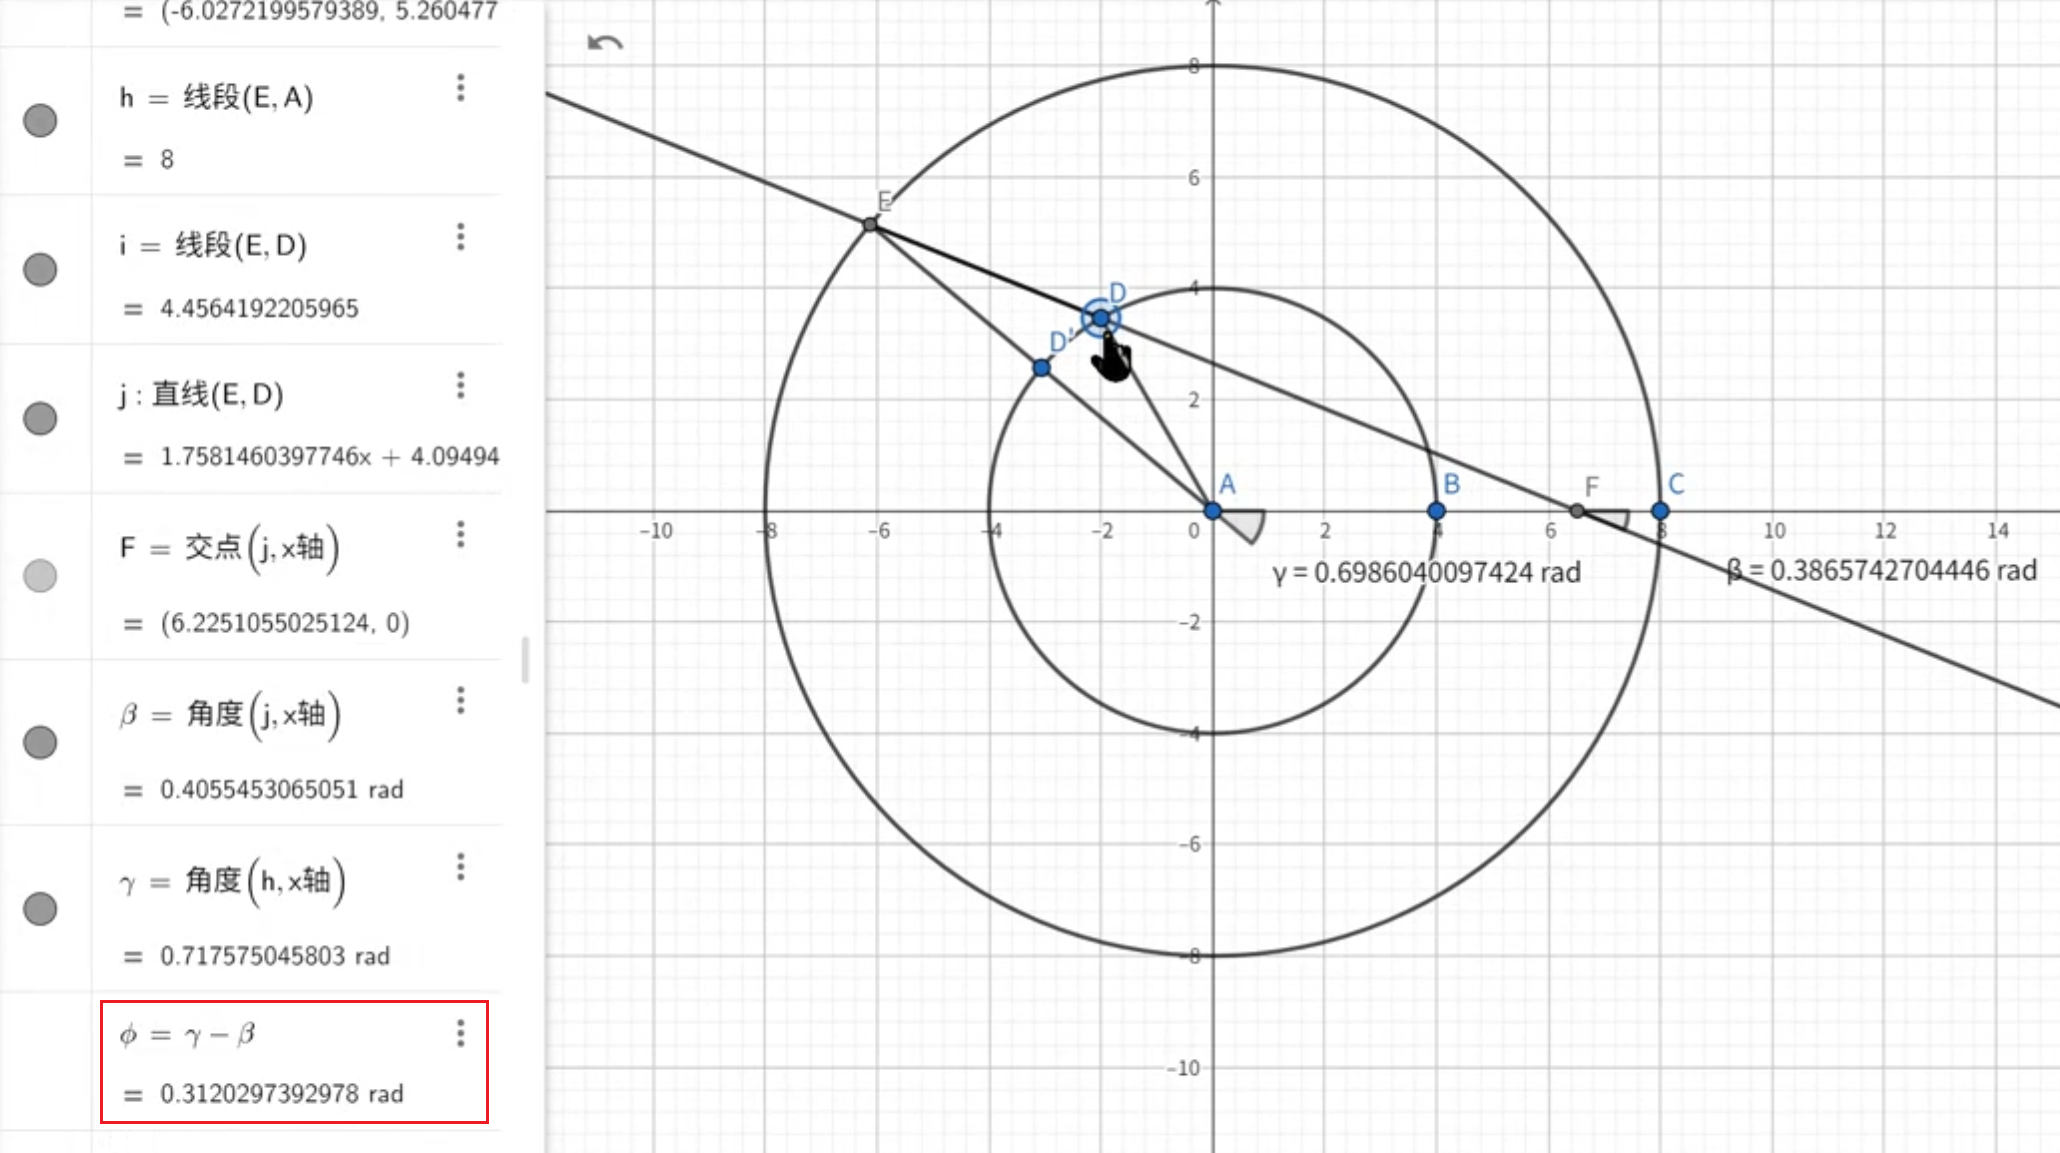
\includegraphics[width=\linewidth]{Figs/1.png}
    \end{minipage}
    \hfill
    \begin{minipage}[t]{0.48\textwidth}
        \centering
        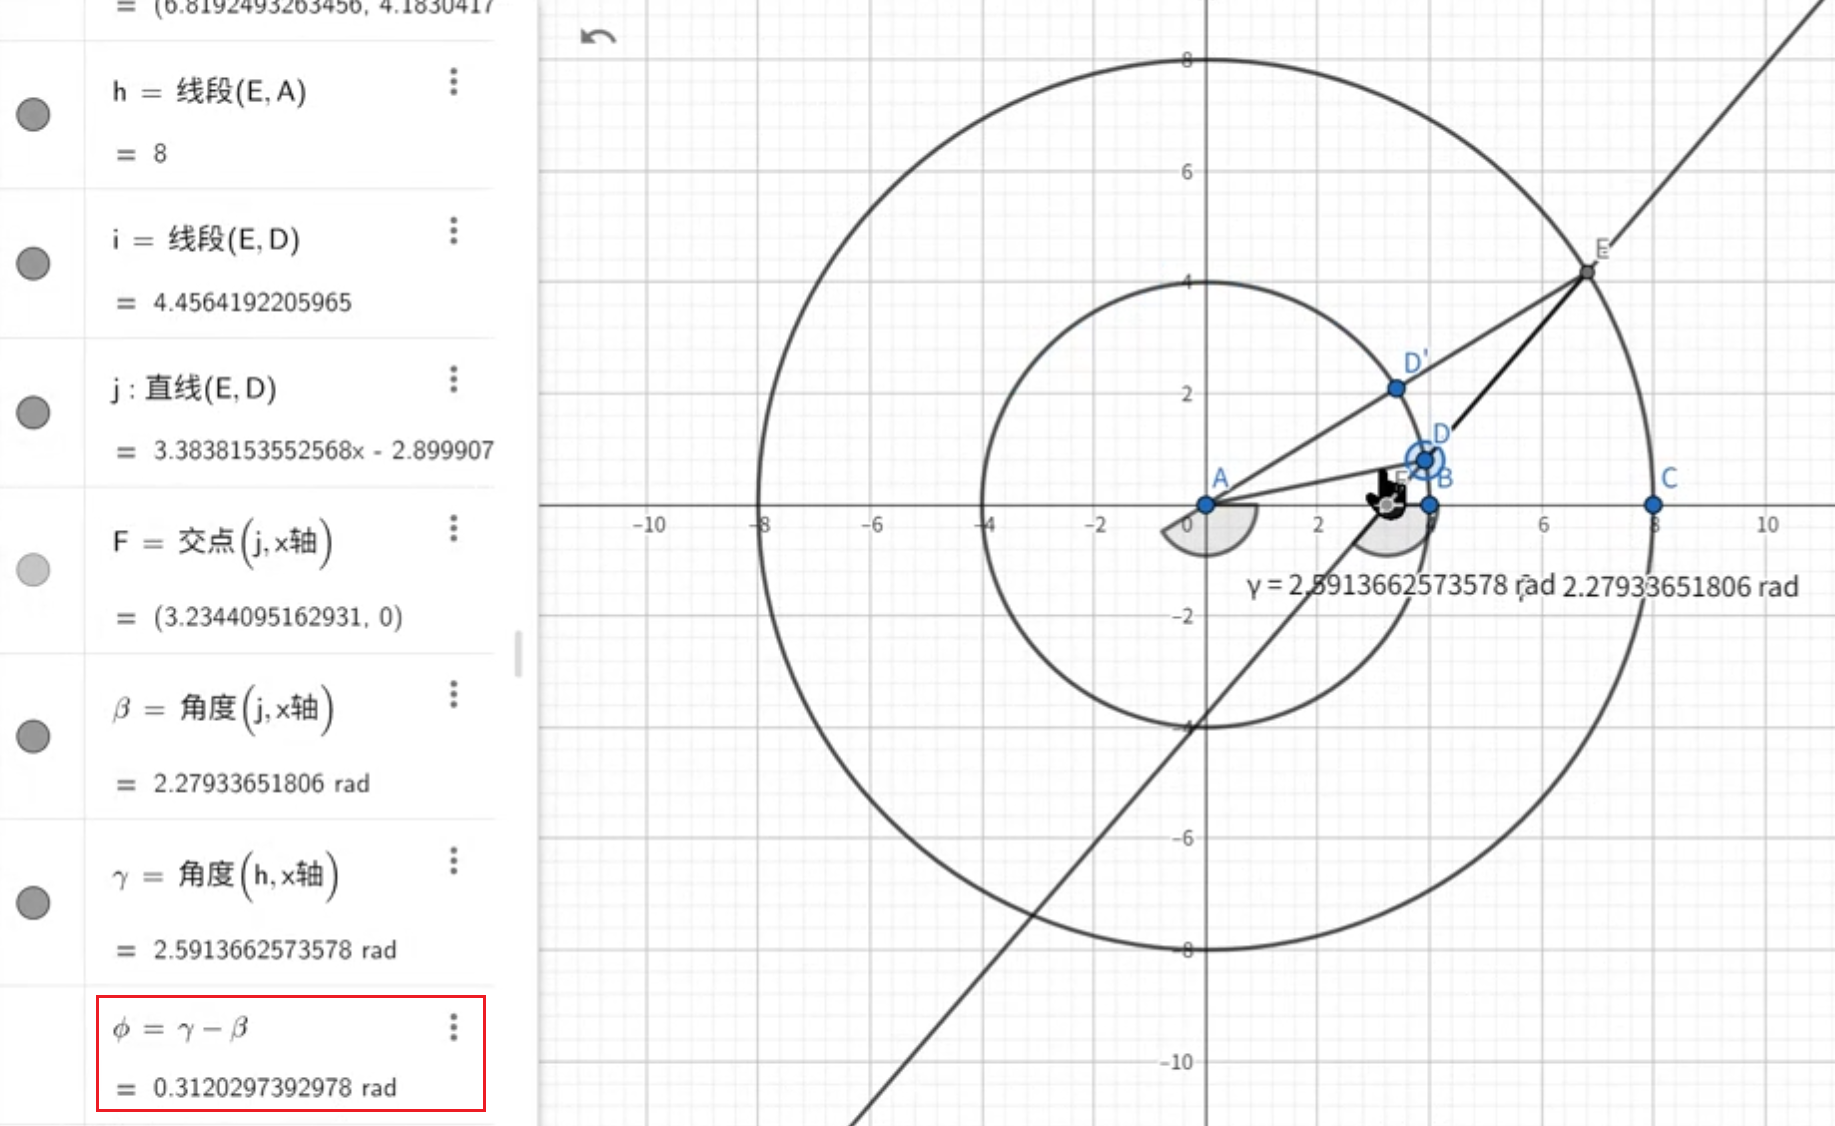
\includegraphics[width=\linewidth]{Figs/2.png}
    \end{minipage}
\end{figure}

得到$\theta(t)$的表达式之后,由于已知质心做球面摆运动,可以写出质心的横纵坐标-时间公式:

$$\left\{
\begin{aligned}
    x_c(t)&=x_{c_0}+a\cos(\omega_{g}t+\varphi_x) \\
    y_c(t)&=y_{c_0}+b\sin(\omega_{g}t+\varphi_y)
\end{aligned}
\right.$$

将$x_c(t),y_c(t)$的表达式代入,结合得到的$\theta(t)$的表达式,拟合:

$$\left\{
\begin{aligned}
    x_1(t)&=x_{c_0}+a\cos(\omega_{g}t+\varphi_x)+R_1\cos(\theta(t)+\theta_x) \\
    y_1(t)&=y_{c_0}+b\sin(\omega_{g}t+\varphi_y)+R_1\sin(\theta(t)+\theta_y)
\end{aligned}
\right.$$
$$\left\{
\begin{aligned}
    x_2(t)&=x_{c_0}+a\cos(\omega_{g}t+\varphi_x)+R_2\cos(\theta(t)+\theta_x) \\
    y_2(t)&=y_{c_0}+b\sin(\omega_{g}t+\varphi_y)+R_2\sin(\theta(t)+\theta_y)
\end{aligned}
\right.$$

分别对做四组拟合,其中$\theta(t)$是一个已知量,由$\theta(t)=\arctan\dfrac{y_2(t)-y_1(t)}{x_2(t)-x_1(t)}$计算得出。

而$x_{c_0},y_{c_0},a,b,R_1,R_2,\omega_{g},\theta_1,\theta_2,\varphi_1,\varphi_2$则是拟合参数,这些物理量的物理意义为:

$x_{c_0},y_{c_0}$是质心运动轨迹形成的椭圆的中心坐标;$a,b$是质心运动轨迹形成的椭圆在$x,y$轴上的投影长度的一半,大于$0$;$R_1,R_2$是$A,B$两点到质心的距离,大于$0$;$\theta_1,\theta_2$是$A,B$点扭摆运动的修正角;$\varphi_x,\varphi_y$是质心球面摆运动的修正角。

拟合完成后,带入表达式,就得到了$x_1(t),y_1(t),x_2(t),y_2(t)$的表达式。

添加圆盘后,由于圆盘是中心对称并且认为其质量均匀分布,故可以认为添加圆盘前后质心的水平位置不会变化。

得到结果后进行比较:转动惯量只影响扭摆的圆频率,根据公式:

$$
\text{扭摆:}\omega=\sqrt{\dfrac{\kappa}{I}}
$$

其中$\kappa$是定值,所以$w$和$I$成平方反比关系。

\section*{四、实验内容}

\begin{enumerate}
    \item 仪器调整
    
    将扭摆仪器置于水平台面,检查台面是否水平,防止出现竖直方向上的运动,干扰实验。调整扭摆摆线钢丝至合适长度,使拍摄视频的工作便于进行。拧紧摆线两端的固定旋钮,避免实验中出现摆长变化。

    \item 拍摄视频
    
    \begin{enumerate}
        \item 拍摄前准备:用黑色马克笔在刚体上标记两个点,便于后期点的追踪。测量绳长三次并取平均值。手机开启视频录制模式,对焦在刚体上。将手机调整到合适的放大倍数,使得两个标记点清晰可见,并且转动过程中不会离开屏幕范围;
        \item 开始视频录制,将手机水平放置于扭摆底座上。轻轻扭转旋钮并推动刚体,使其开始运动,待其运动平稳后录制,得到一个$30-40\,s$的$30fps$视频。注意在视频拍摄的过程中不要移动扭摆实验仪器;
        \item 不改变摆线长度,在刚体上增加一个圆环,重复上述步骤,得到第二个视频。
    \end{enumerate}
    
    \item 数据处理
    
    \begin{enumerate}
        \item 将视频导入tracker软件,选择两个标记点(即马克笔标记的两个黑色点),进行自动追踪,得到两组点的横纵坐标-时间数据;
        \item 将数据导入Origin,Matlab进行数据分析,得到$\theta(t),x_1(t),y_1(t),x_2(t),y_2(t)$坐标的函数表达式,\\
        对$x_{c_0},y_{c_0},A,R_1,R_2,\omega_{g},\theta_1,\theta_2,\varphi_1,\varphi_2$等拟合参数的拟合值,绘制相关图像。
    \end{enumerate}

\end{enumerate}

\section*{五、数据记录}

\begin{tabular}{|c|c|c|c|c|}
    \hline
      & 1   & 2   & 3   & 平均 \\
    \hline
    绳长 L/m & 0.5781 & 0.5782 & 0.5786 & 0.5783 \\
    \hline
\end{tabular}

其余数据均为视频录像。

\section*{六、数据处理}

\begin{enumerate}
    \item 不添加刚体圆环:
    \begin{enumerate}
        \item 拟合$\theta(t)$:由公式$\theta(t)=\arctan\dfrac{y_2(t)-y_1(t)}{x_2(t)-x_1(t)}$可以得到每个时间对应的$\theta(t)$,将$\theta(t)$的计算结果进行拟合,拟合公式为:$\theta(t)=\theta_0+A\sin(\omega t+\varphi)$得到:$\theta(t)=0.1095+1.3457\sin(1.1947t-0.3022)$。下面是得到的$\theta(t)$拟合图:

        \begin{figure}[H]
            \centering
            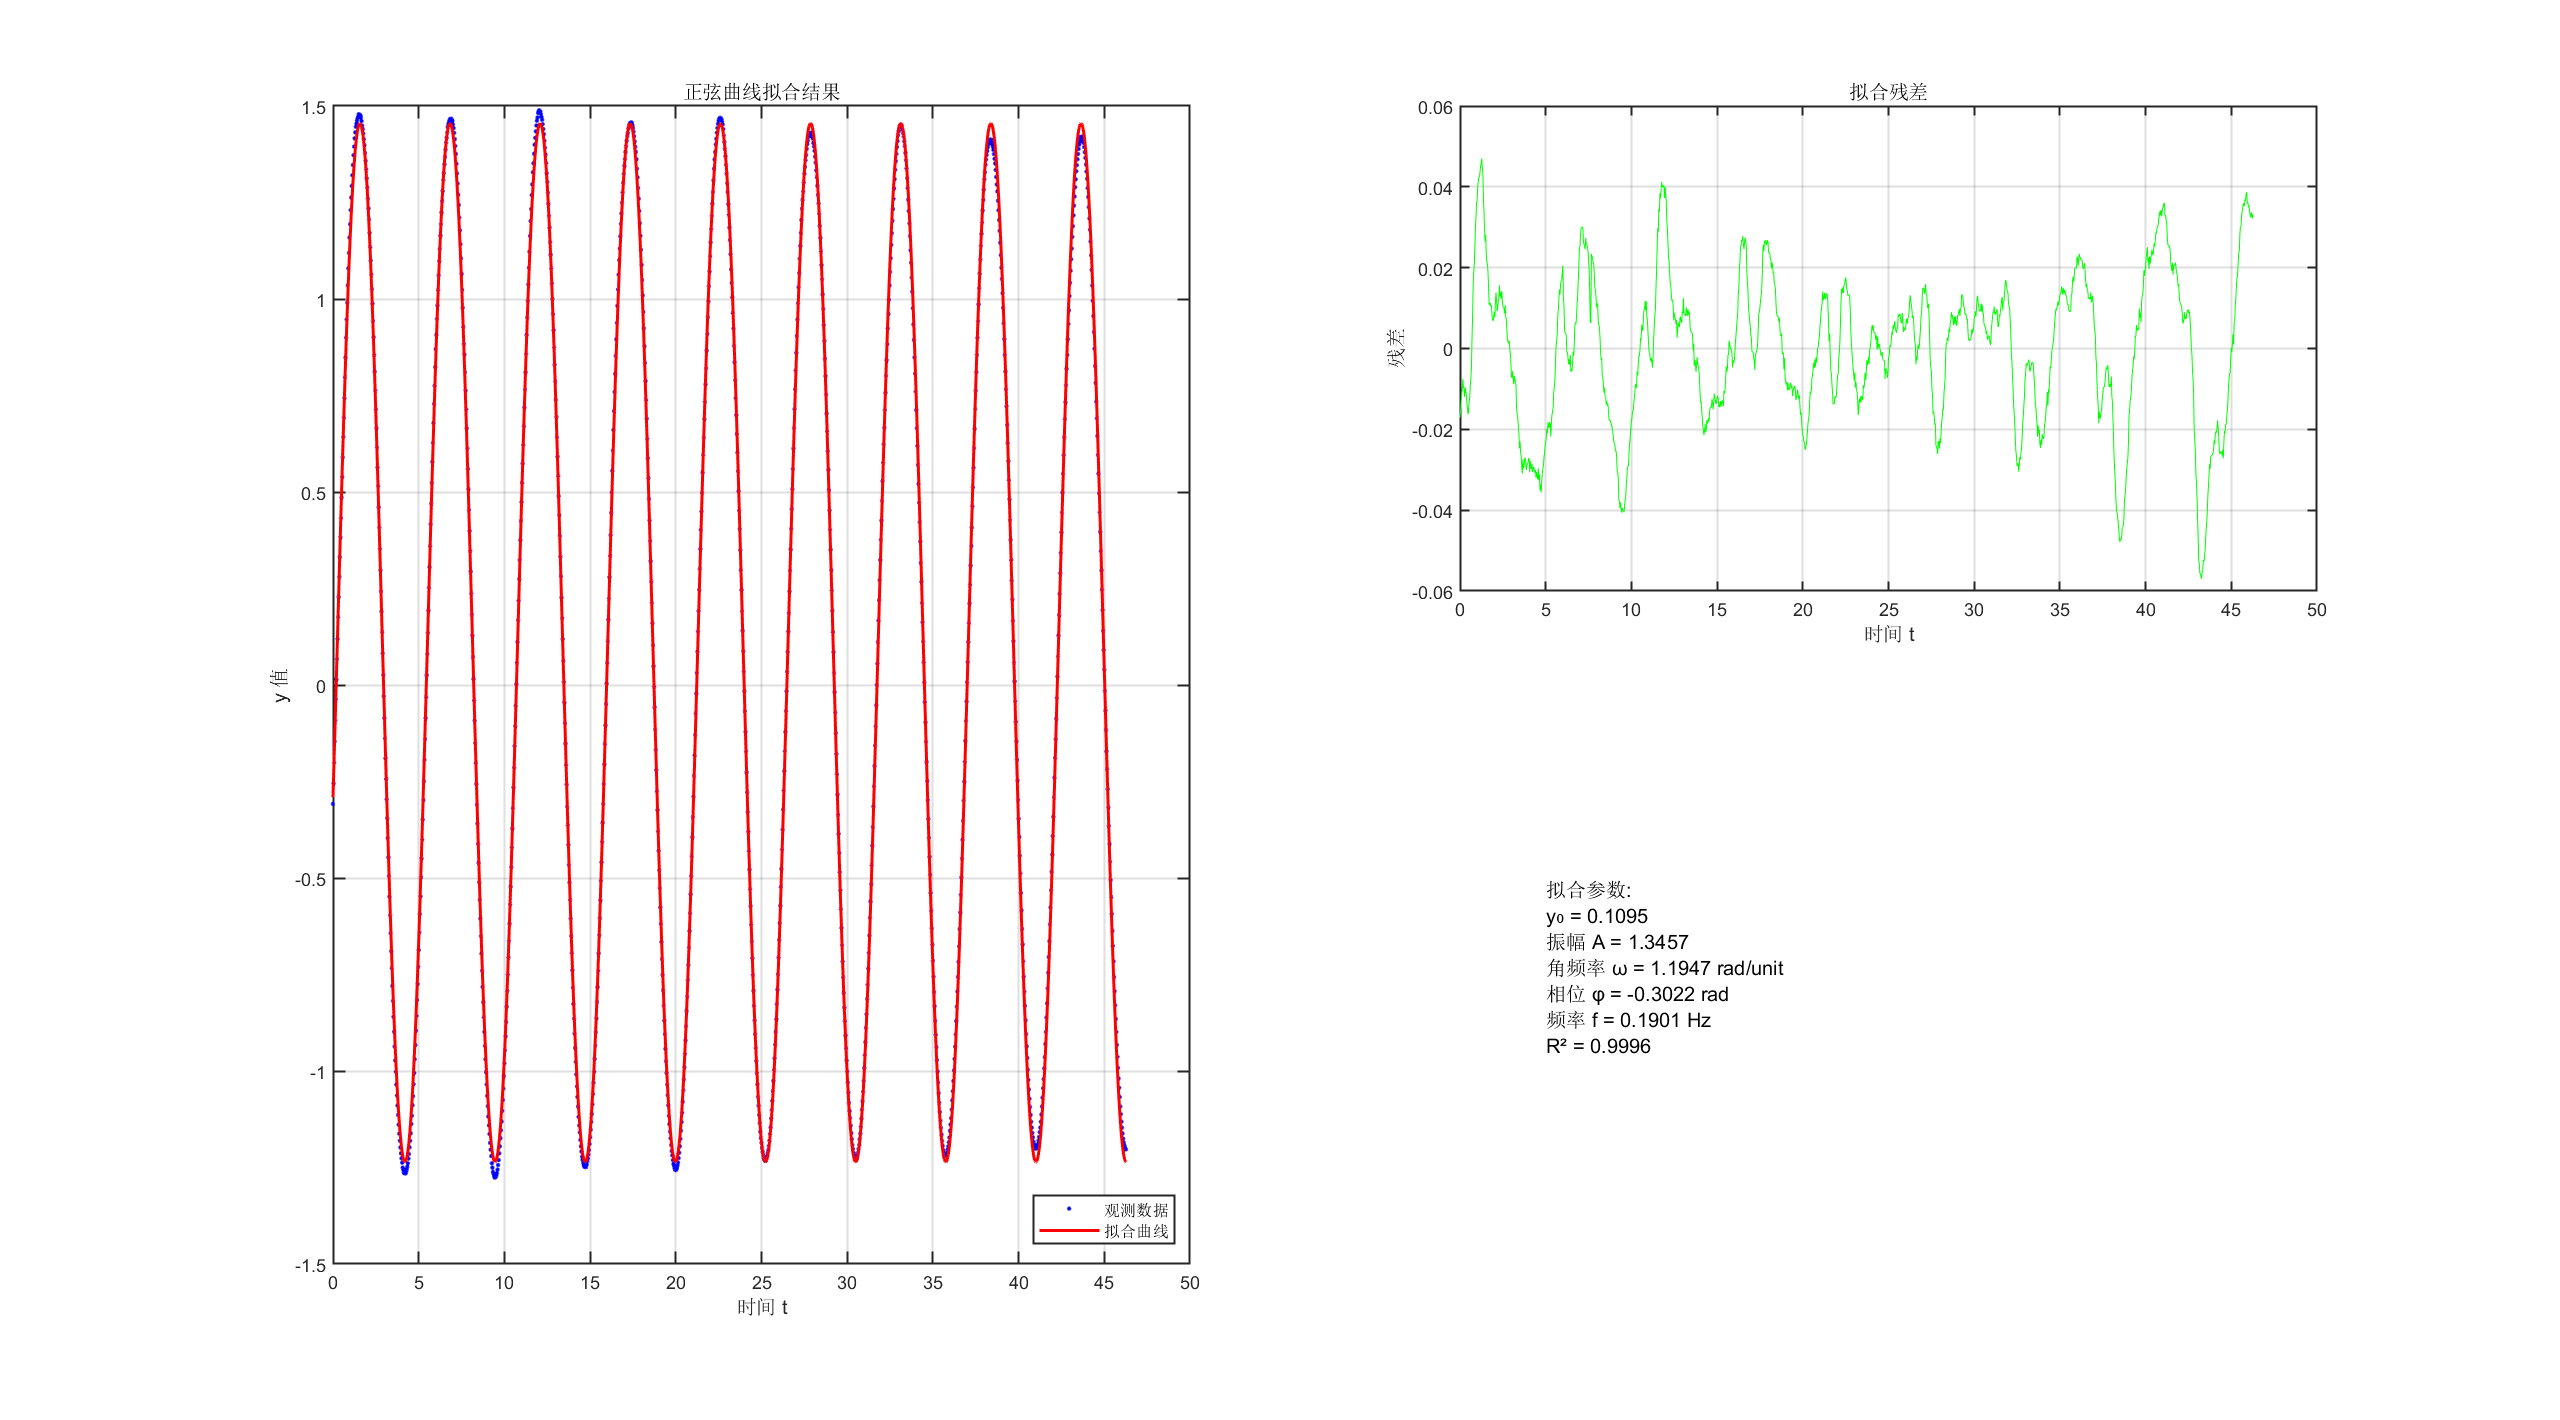
\includegraphics[width=0.9\textwidth]{Figs/Ex1.theta.png}
            \caption{$\theta(t)$拟合图}
        \end{figure}
        \item 拟合$x_{c_0},y_{c_0},a,b,R_1,R_2,\omega_{g},\theta_1,\theta_2,\varphi_1,\varphi_2$,得到$x_1(t),y_1(t),x_2(t),y_2(t)$的表达式:

        $$\left\{
        \begin{aligned}
            x_1(t)&=x_{c_0}+a\cos(\omega_{g}t+\varphi_x)+R_1\cos(\theta(t)+\theta_x) \\
            y_1(t)&=y_{c_0}+b\sin(\omega_{g}t+\varphi_y)+R_1\sin(\theta(t)+\theta_y)
        \end{aligned}
        \right.$$
        $$\left\{
        \begin{aligned}
            x_2(t)&=x_{c_0}+a\cos(\omega_{g}t+\varphi_x)+R_2\cos(\theta(t)+\theta_x) \\
            y_2(t)&=y_{c_0}+b\sin(\omega_{g}t+\varphi_y)+R_2\sin(\theta(t)+\theta_y)
        \end{aligned}
        \right.$$

        将$\theta(t)=0.1095+1.3457\sin(1.1947t-0.3022)$带入,进行拟合,进行三角诱导公式使得$R_1>0$,得到:

        $$\left\{
        \begin{aligned}
            x_1&=58.3069+57.9607\cos(4.1060t-1.2094)+106.5522\cos(\theta(t)+3.0807) \\
            y_1&=-334.7360+82.3392\sin(4.1060t-3.0593)+106.5522\sin(\theta(t)+3.1023)
        \end{aligned}
        \right.$$
        $$\left\{
        \begin{aligned}
            x_2&=57.8732+57.2387\cos(4.1061t-1.2152)+108.3969\cos(\theta(t)+0.0547) \\
            y_2&=-333.8828+83.0249\sin(4.1061t-3.0724)+108.3969\sin(\theta(t)+0.0343)
        \end{aligned}
        \right.$$
        由拟合结果发现:通过$A$点拟合,椭圆中心在点$(58.3069,-334.7460)$,投射在$x$轴,$y$轴长度的一半分别为$57.9607,82.3392$;通过$B$点拟合,椭圆中心在点$(57.8732,-333.8828)$,投射在$x$轴,$y$轴长度的一半分别为$57.2387,83.0249$。椭圆中心横坐标相对误差为$\left|\frac{57.8732-58.3069}{58.3069}\right|\times100\%=0.744\% $;椭圆中心纵坐标相对误差为$\left|\frac{-333.8828-(-334.7360)}{-334.7360}\right|\times100\%=0.255\%$;投射在$x$轴长度的一半的相对误差为$\left|\frac{57.2387-57.9607}{57.9607}\right|\times100\%=1.246\%$;投射在$y$轴长度的一半的相对误差为$\left|\frac{83.0249-82.3392}{82.3392}\right|\times100\%=0.833\%$。四者差距均很小,故可认为两点所构成的质点椭圆轨迹近似相同,进一步验证实验准确性以及实验假设。
        
        下面是得到的拟合参数和$A,B$两点的横纵坐标-时间拟合图:

        \begin{figure}[H]
            \centering
            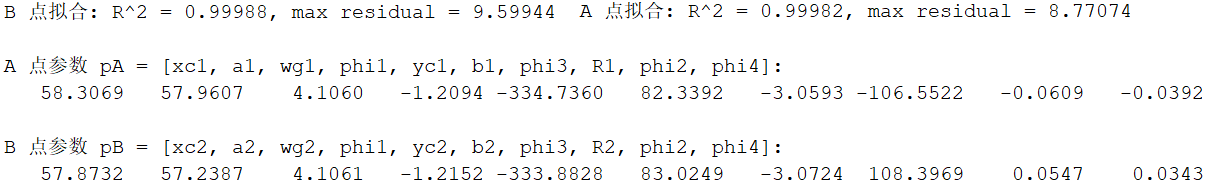
\includegraphics[width=0.9\textwidth]{Figs/Ex1.nums.png}
            \caption{拟合参数}
        \end{figure}
        \vspace{-0.7cm}
        \begin{figure}[H]
            \centering
            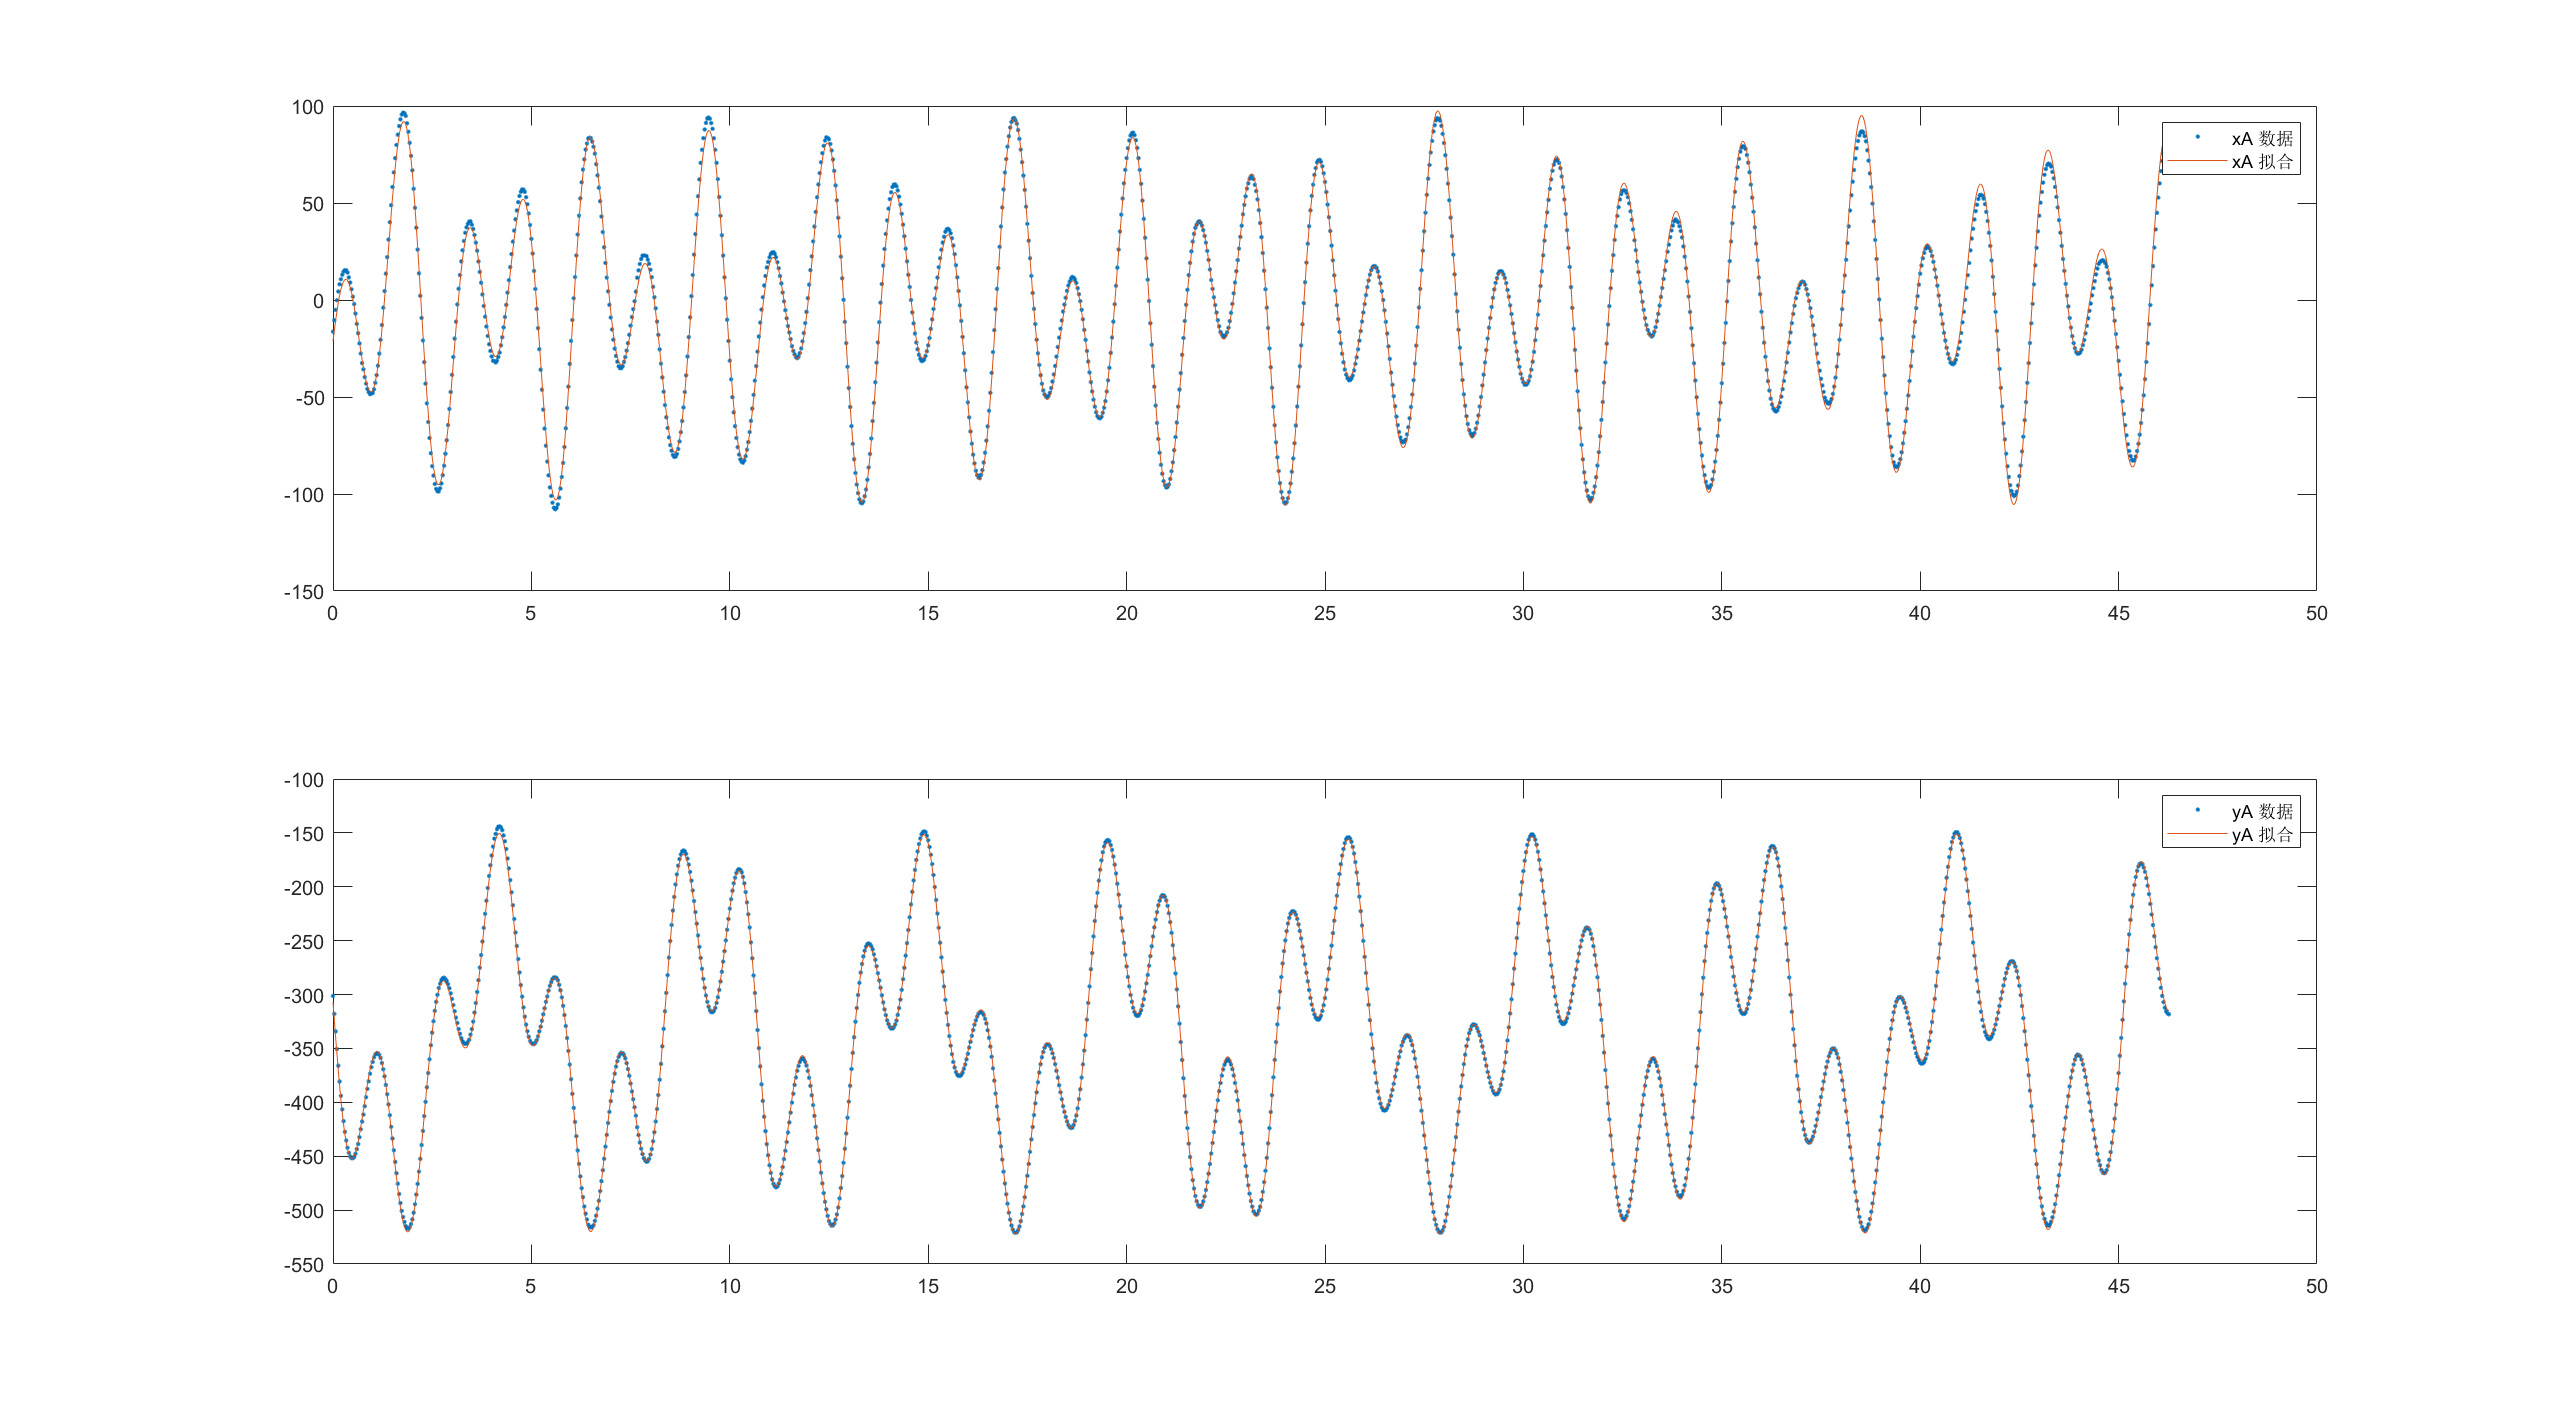
\includegraphics[width=0.9\textwidth]{Figs/Ex1.A.png}
            \vspace{-0.5cm}
            \caption{$A$点横纵坐标-时间拟合图}
        \end{figure}
        \vspace{-0.7cm}
        \begin{figure}[H]
            \centering
            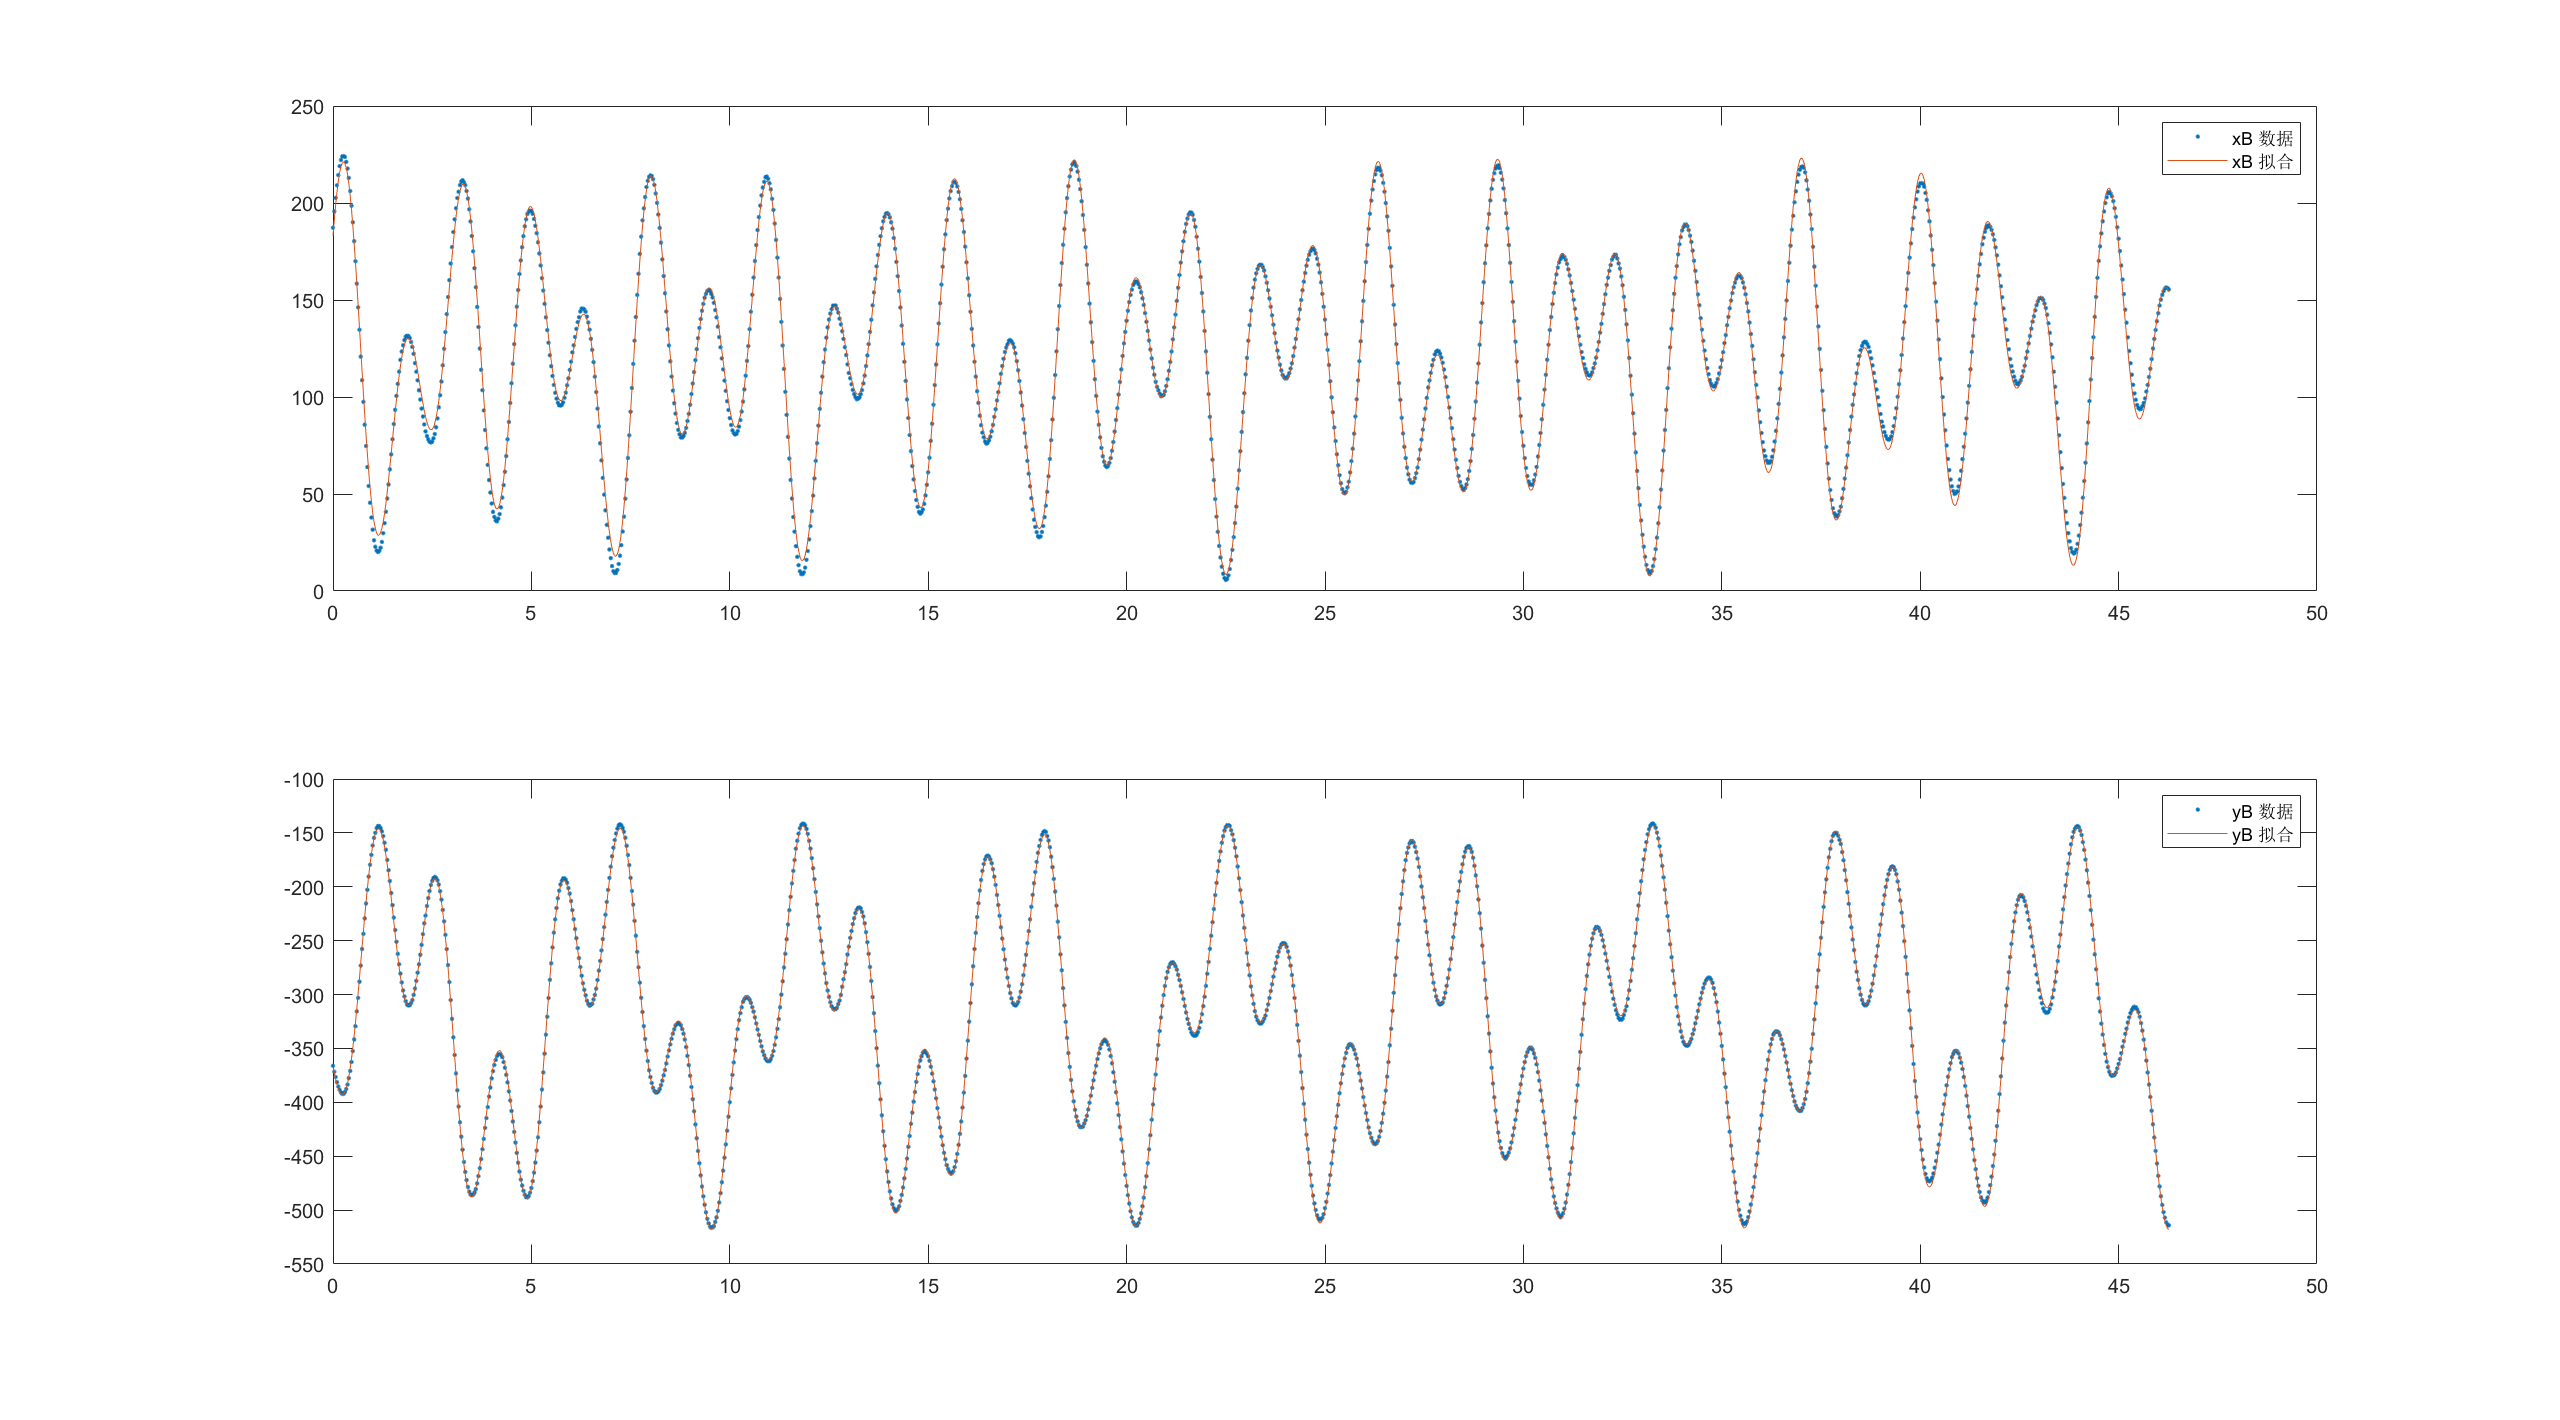
\includegraphics[width=0.9\textwidth]{Figs/Ex1.B.png}
            \vspace{-0.5cm}
            \caption{$B$点横纵坐标-时间拟合图}
        \end{figure}
        
        \item 将得到的拟合参数带入公式$(1),(2),(3),(4)$,由$A,B$两点运动轨迹去除扭摆运动轨迹,反推得到两组$(x_c(t),y_c(t))$的坐标轨迹你函数,绘图得到:
        
        \begin{figure}[H]
            \centering
            \begin{minipage}[t]{0.48\textwidth}
                \centering
                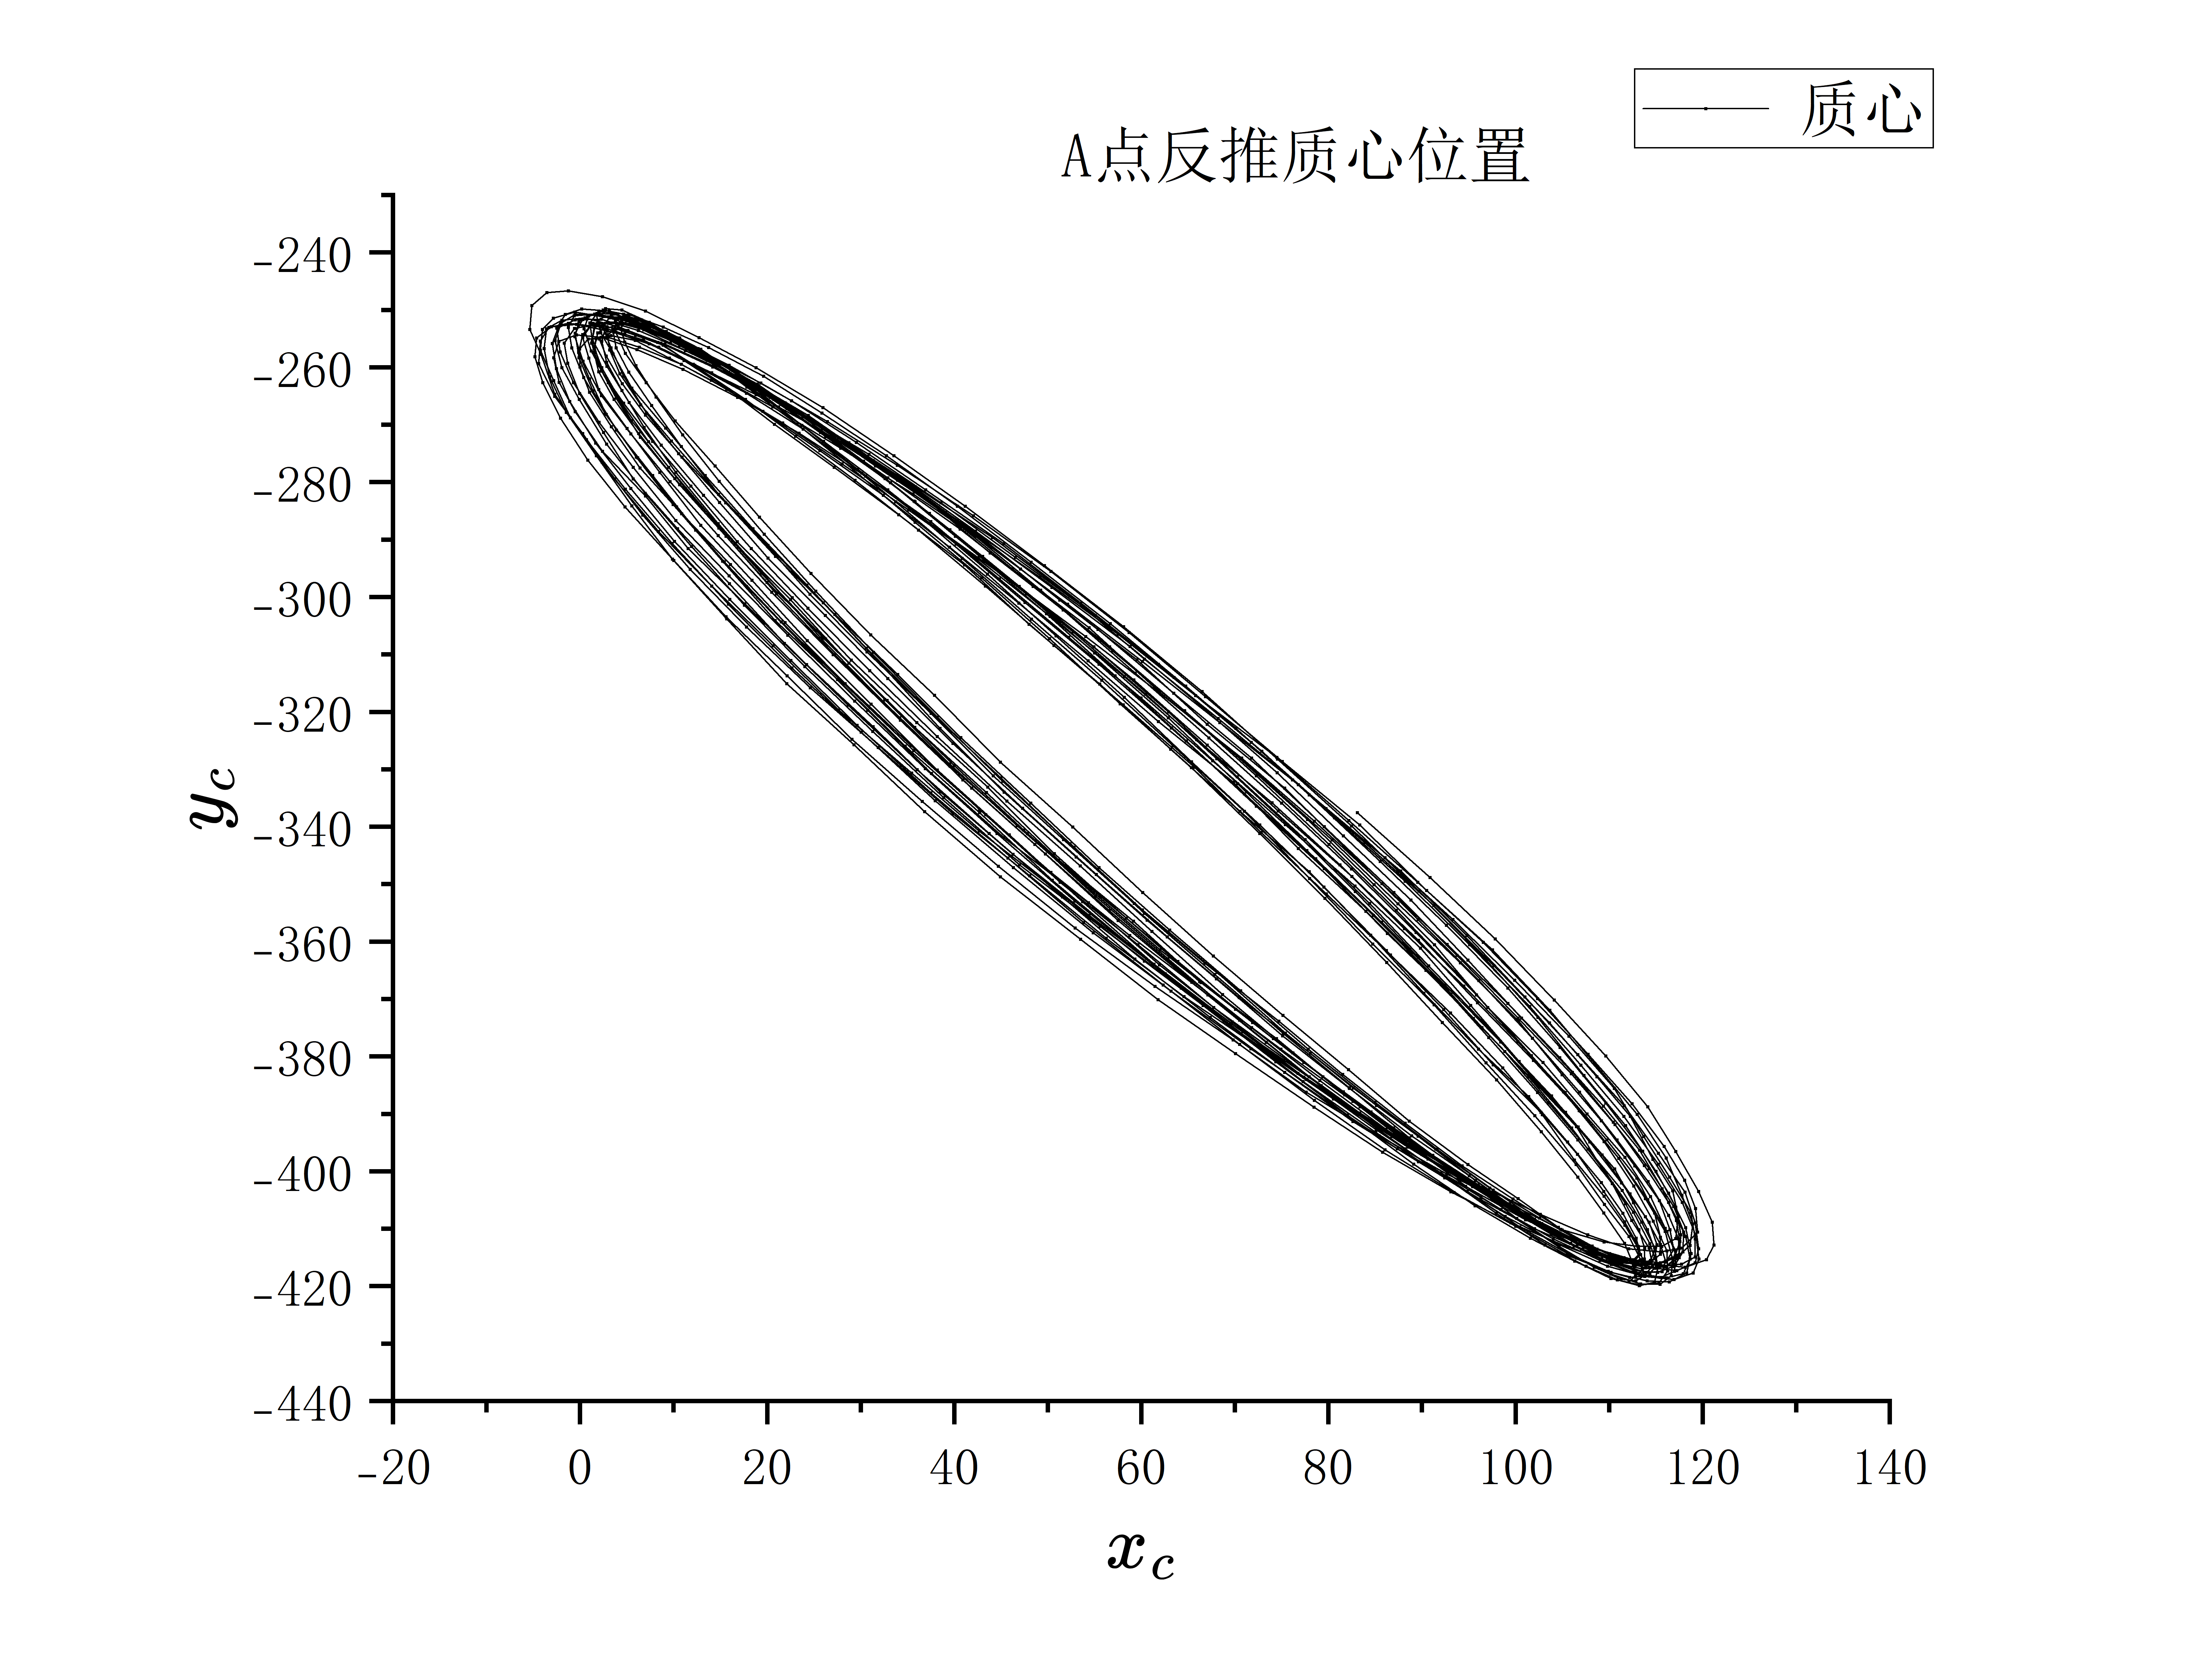
\includegraphics[width=\linewidth]{Figs/Ex1.A.c.png}
                \vspace{-0.5cm}
                \caption{$A$点反推的质心坐标轨迹图}
            \end{minipage}
            \hfill
            \begin{minipage}[t]{0.48\textwidth}
                \centering
                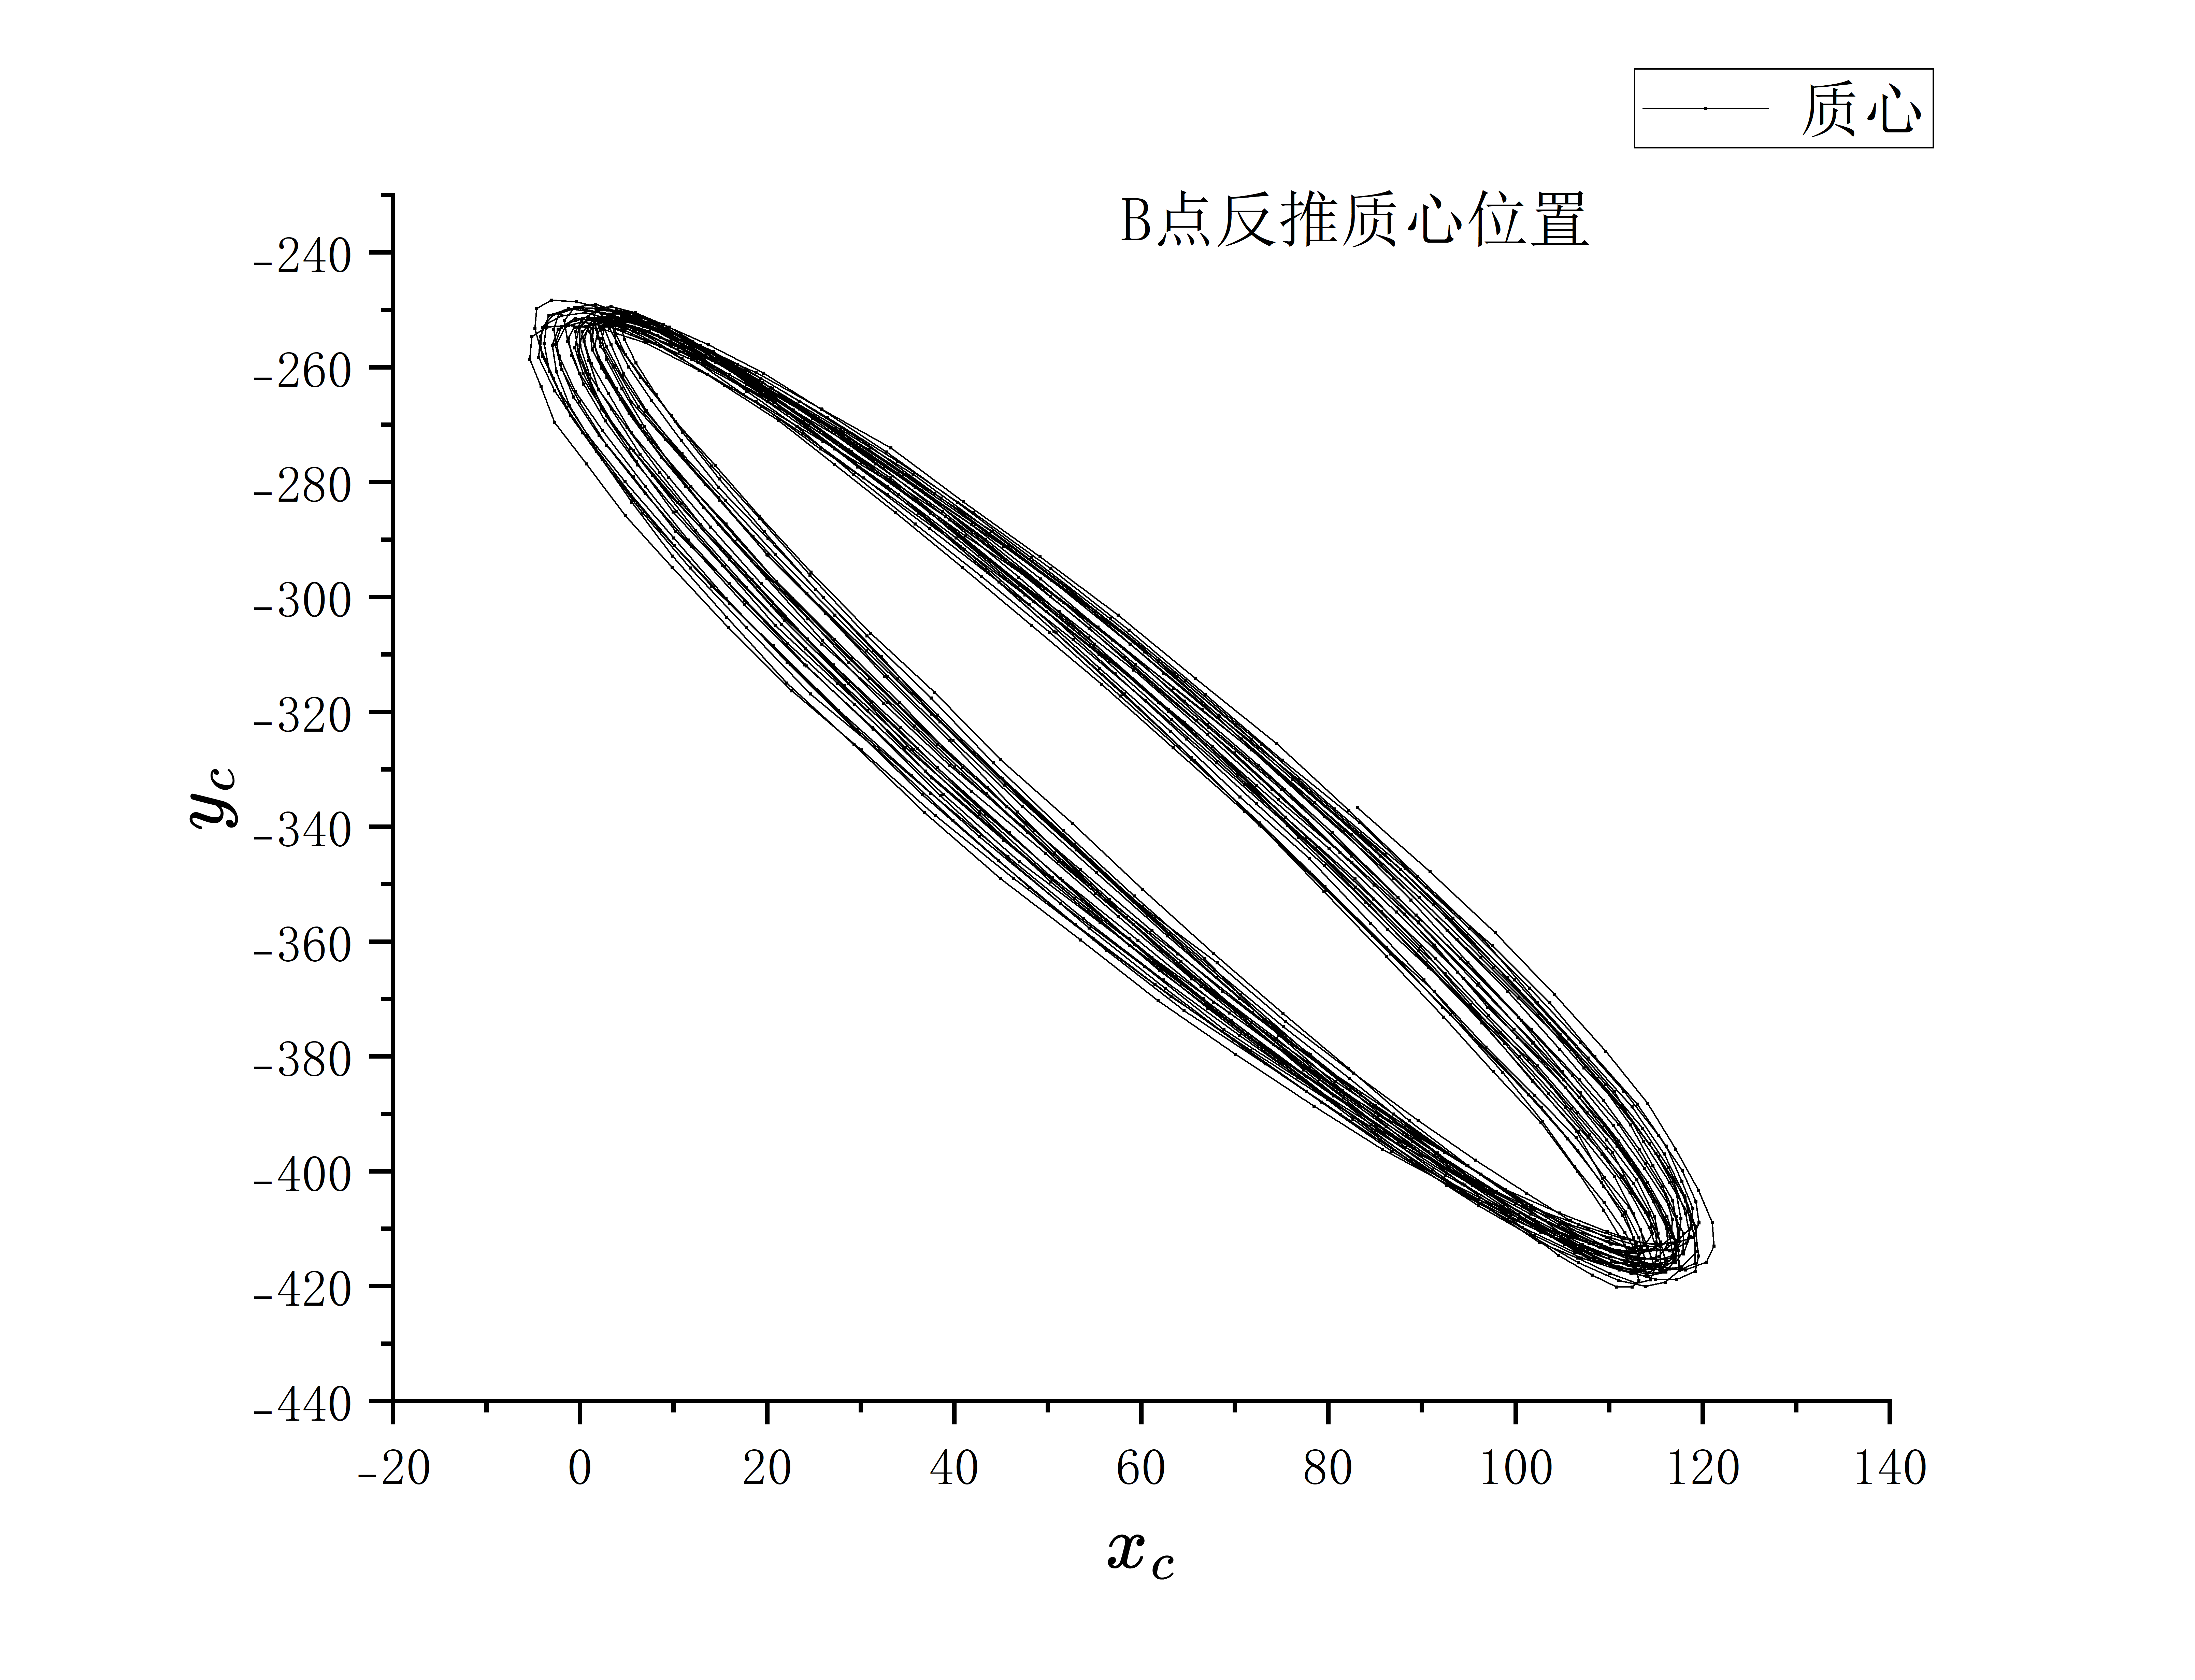
\includegraphics[width=\linewidth]{Figs/Ex1.B.c.png}
                \vspace{-0.5cm}
                \caption{$B$点反推的质心坐标轨迹图}
            \end{minipage}
        \end{figure}
    \end{enumerate}
    \item 添加刚体圆环:
    \begin{enumerate}
        \item 拟合$\theta(t)$,得到:$\theta(t)=-0.9045+0.4808\sin(0.7048t-0.6891)$。下面是得到的$\theta(t)$拟合图:
        \begin{figure}[H]
            \centering
            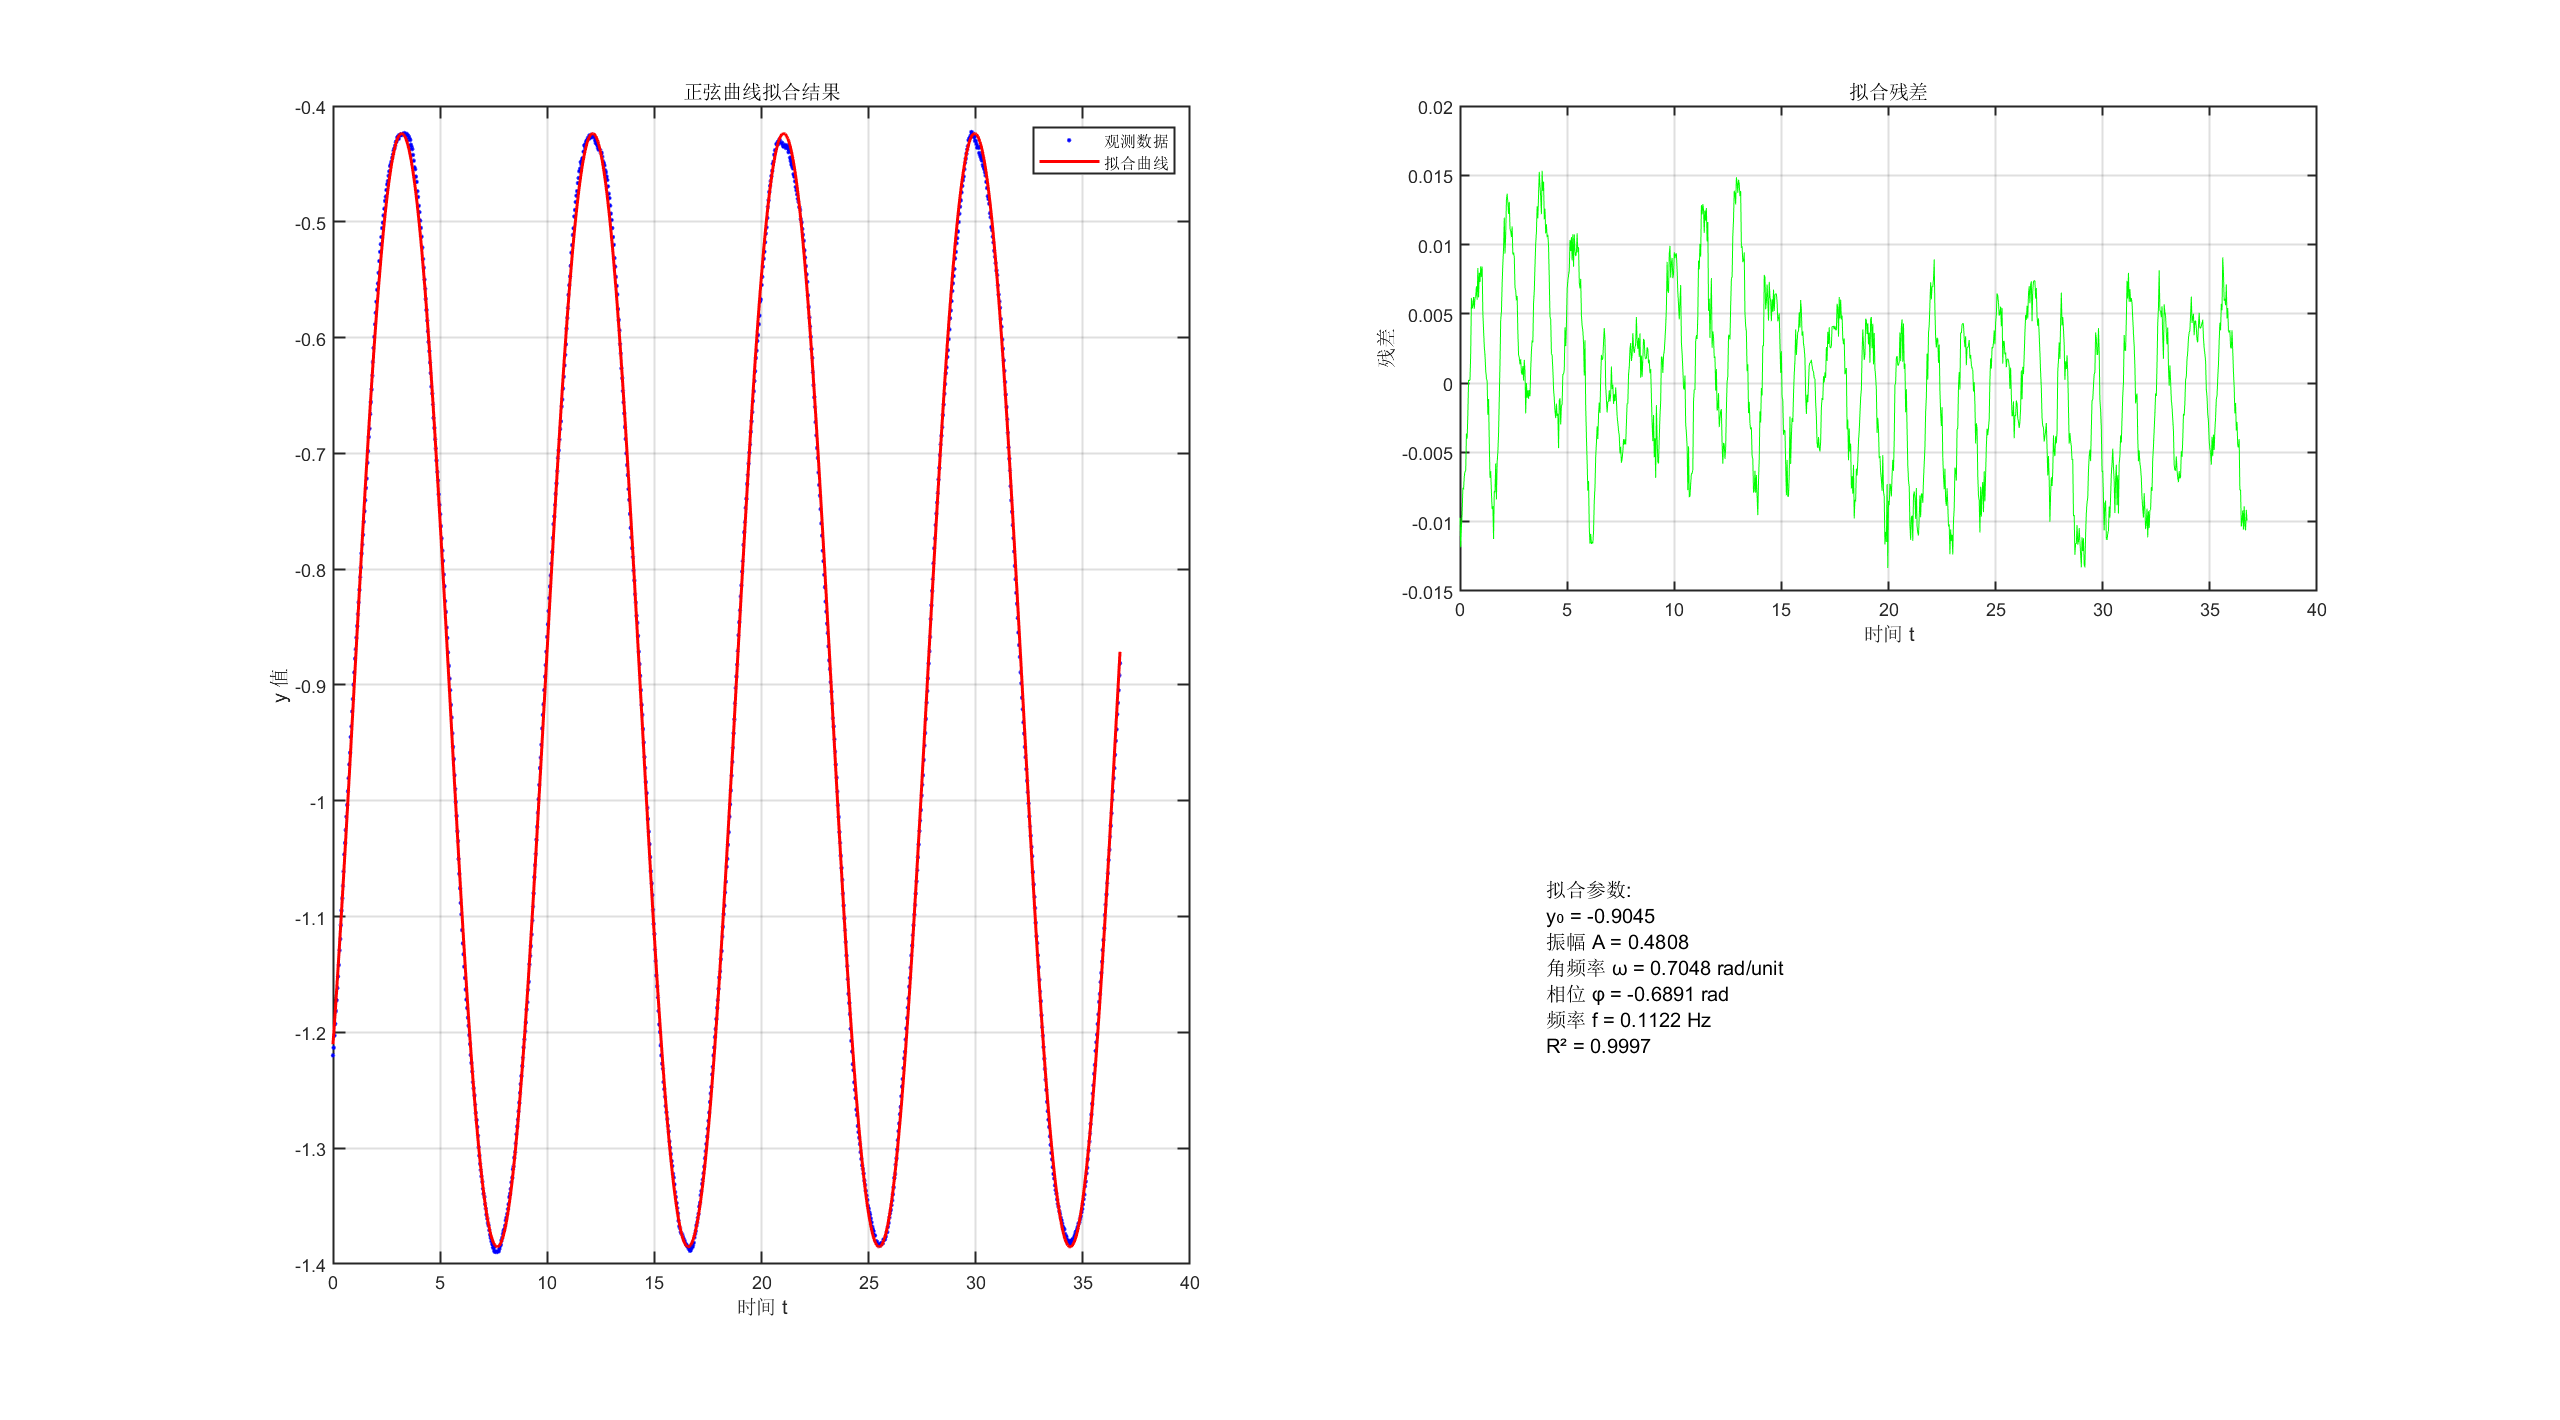
\includegraphics[width=0.8\textwidth]{Figs/Ex2.theta.png}
            \vspace{-0.5cm}
            \caption{$\theta(t)$拟合图}
        \end{figure}
        \item 对$A,B$两点进行拟合,并使用三角诱导公式使得$R_1>0$:
        $$\left\{
        \begin{aligned}
            x_1&=-31.2942+71.1724\cos(4.1178t+2.8592)+91.6279\cos(\theta(t)+3.2592) \\
            y_1&=-447.5730+80.1044\sin(4.1178t+1.9304)+91.6279\sin(\theta(t)+3.2303)
        \end{aligned}
        \right.$$
        $$\left\{
        \begin{aligned}
            x_2&=-28.6870+71.7296\cos(4.1177t+2.8616)+92.7770\cos(\theta(t)-0.1435) \\
            y_2&=-447.2191+78.8005\sin(4.1177t+1.9366)+92.7770\sin(\theta(t)-0.0967)
        \end{aligned}
        \right.$$
        由拟合结果发现:通过$A$点拟合,椭圆中心在点$(-31.2942,-447.5730)$,投射在$x$轴,$y$轴长度的一半分别为$71.1724,80.1044$;通过$B$点拟合,椭圆中心在点$(-28.6870,-447.2191)$,投射在$x$轴,$y$轴长度的一半分别为$71.7296,78.8005$。椭圆中心横坐标相对误差为$\left|\frac{-28.6870-(-31.2942)}{-31.2942}\right|\times100\%=8.331\% $;椭圆中心纵坐标相对误差为$\left|\frac{-447.2191-(-447.5730)}{-447.5730}\right|\times100\%=0.079\%$;投射在$x$轴长度的一半的相对误差为$\left|\frac{71.7296-71.1724}{71.1724}\right|\times100\%=0.783\%$;投射在$y$轴长度的一半的相对误差为$\left|\frac{78.8005-80.1044}{80.1044}\right|\times100\%=1.628\%$。椭圆中心横坐标误差较大,可能是受进动影响,但由于其绝对误差较小,且后三者差距均较小,故可认为两点所构成的质点椭圆轨迹近似相同,进一步验证实验准确性以及实验假设。
        
        下面是得到的拟合参数和$A,B$两点的横纵坐标-时间拟合图:
        \begin{figure}[H]
            \centering
            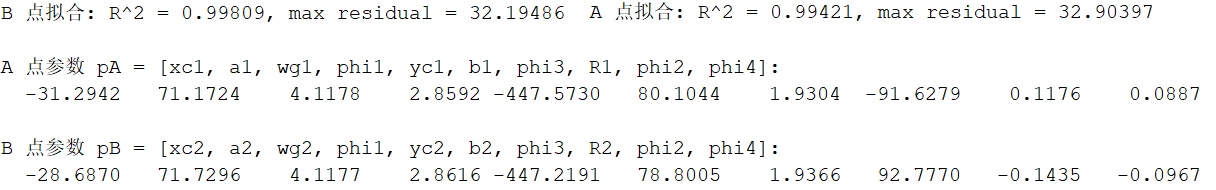
\includegraphics[width=0.9\textwidth]{Figs/Ex2.nums.png}
            \caption{拟合参数}
        \end{figure}
        \vspace{-0.5cm}
        \begin{figure}[H]
            \centering
            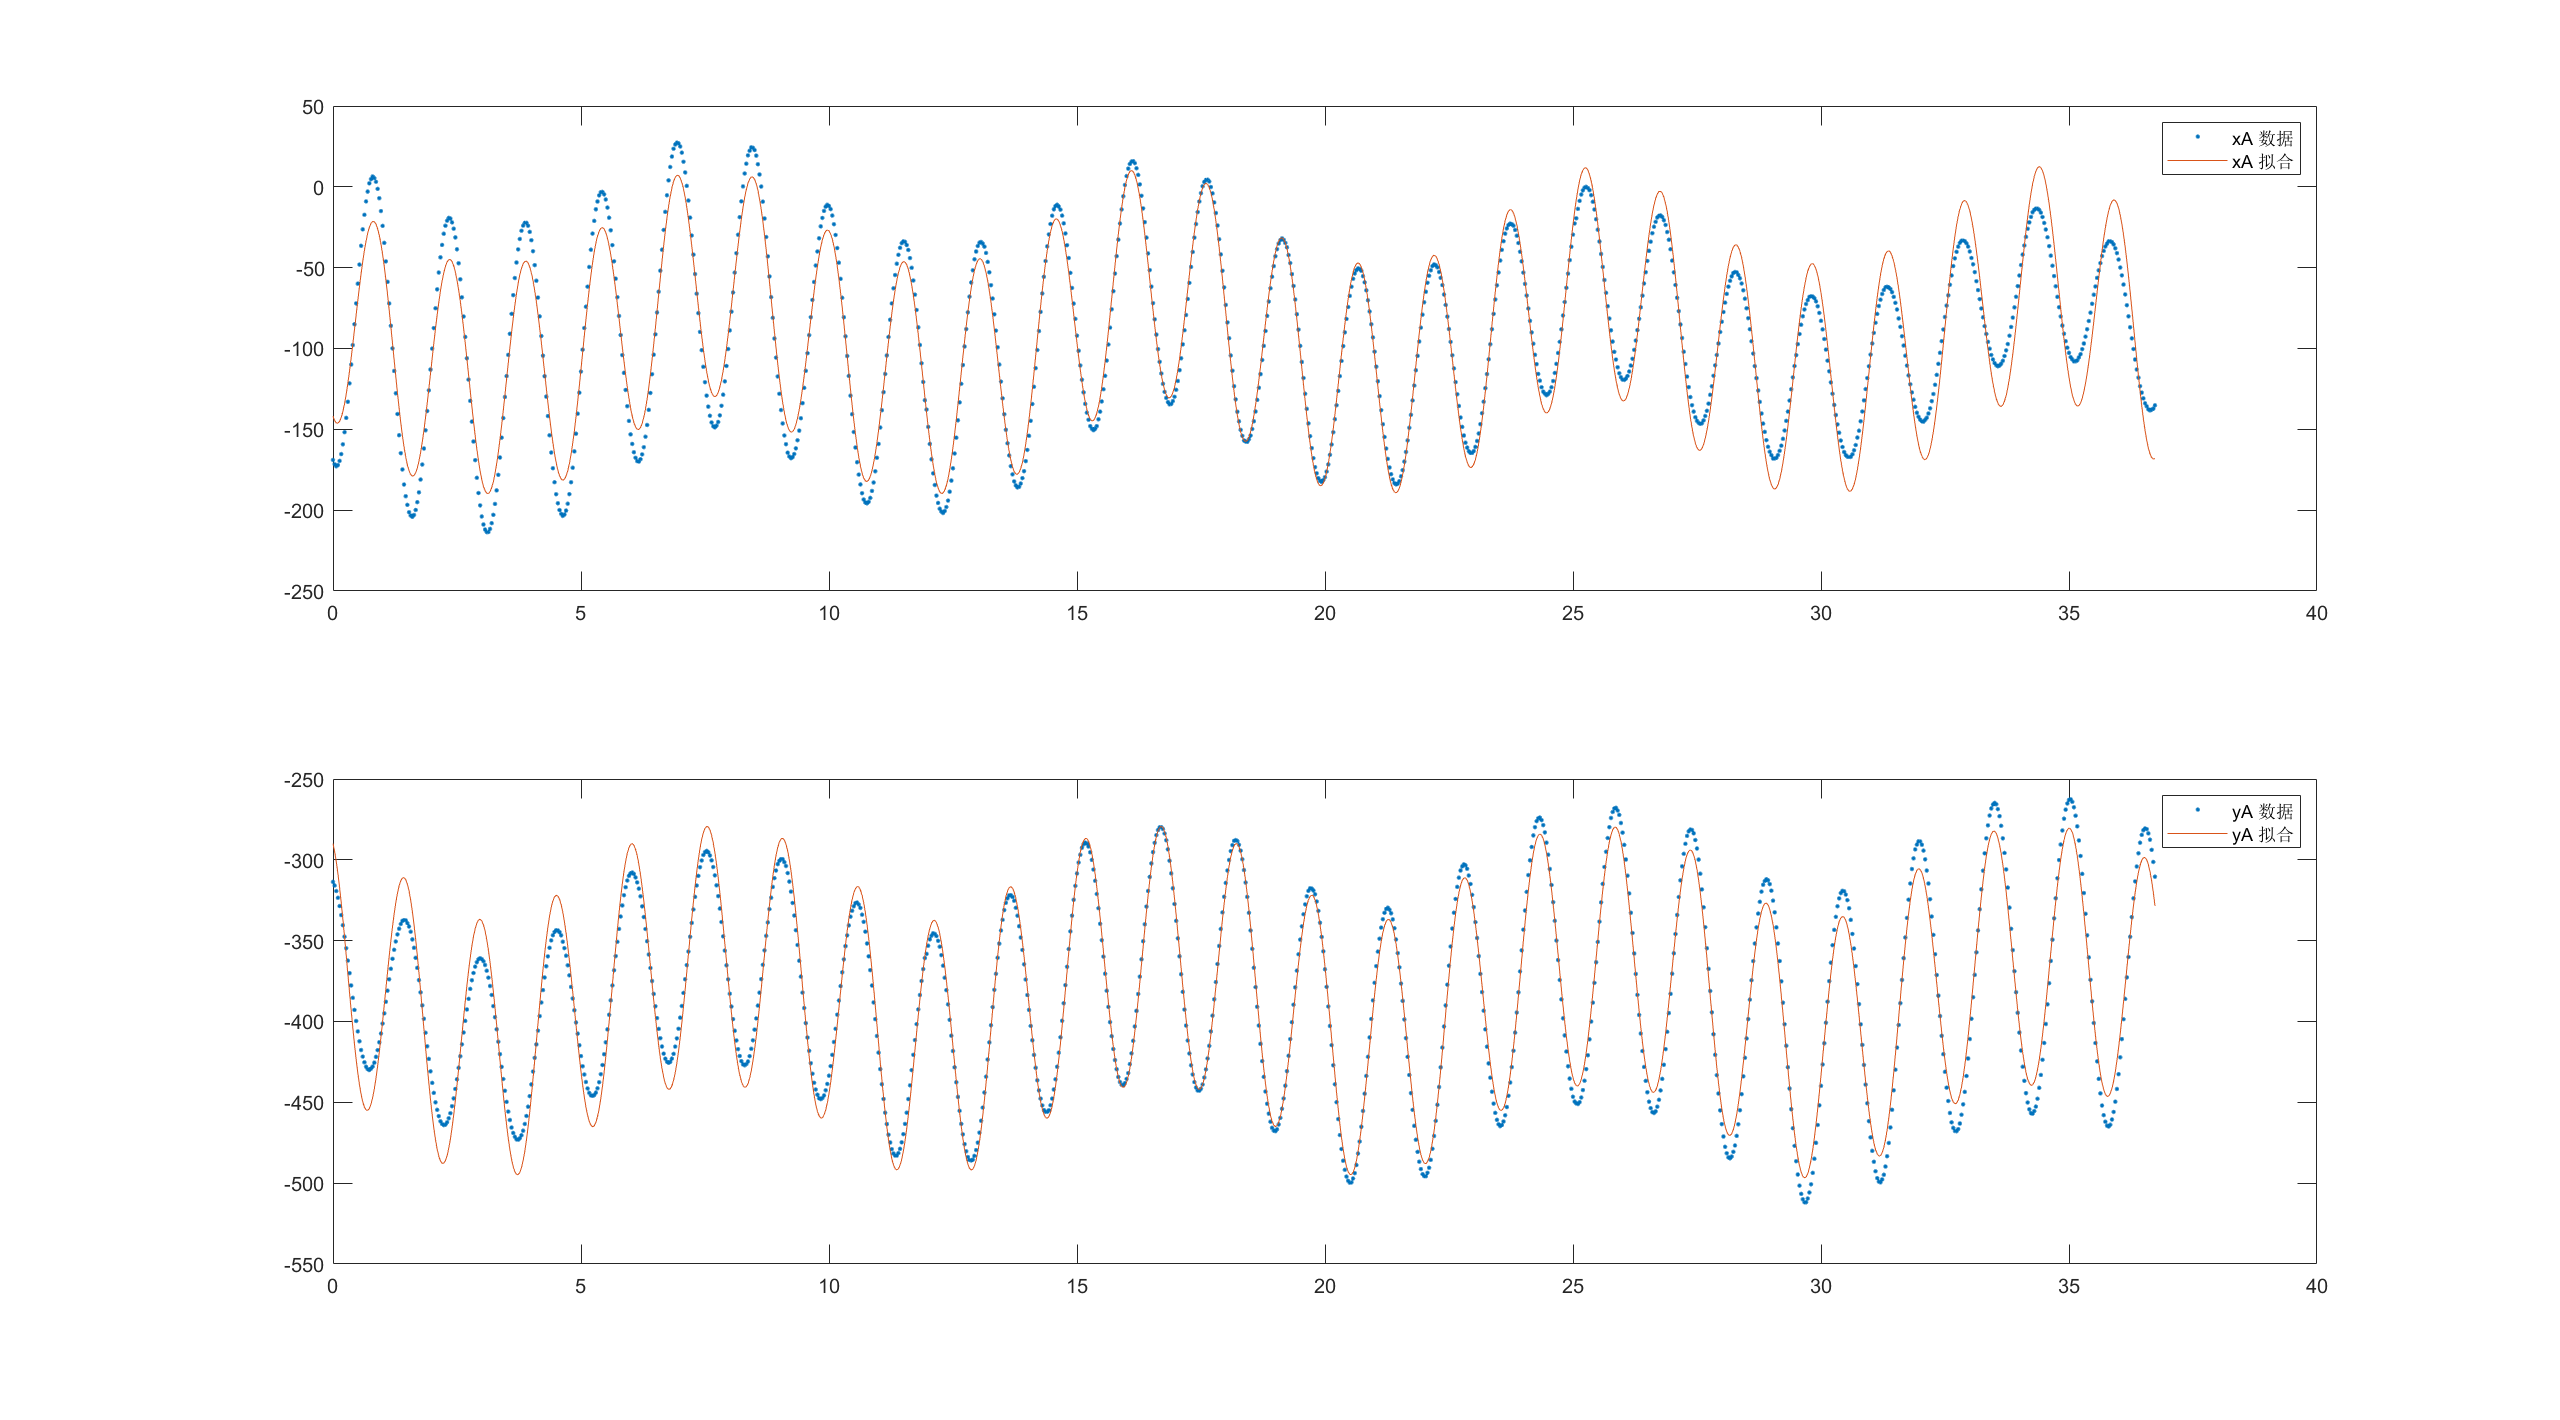
\includegraphics[width=0.9\textwidth]{Figs/Ex2.A.png}
            \vspace{-0.1cm}
            \caption{$A$点横纵坐标-时间拟合图}
        \end{figure}
        \vspace{-0.5cm}
        \begin{figure}[H]
            \centering
            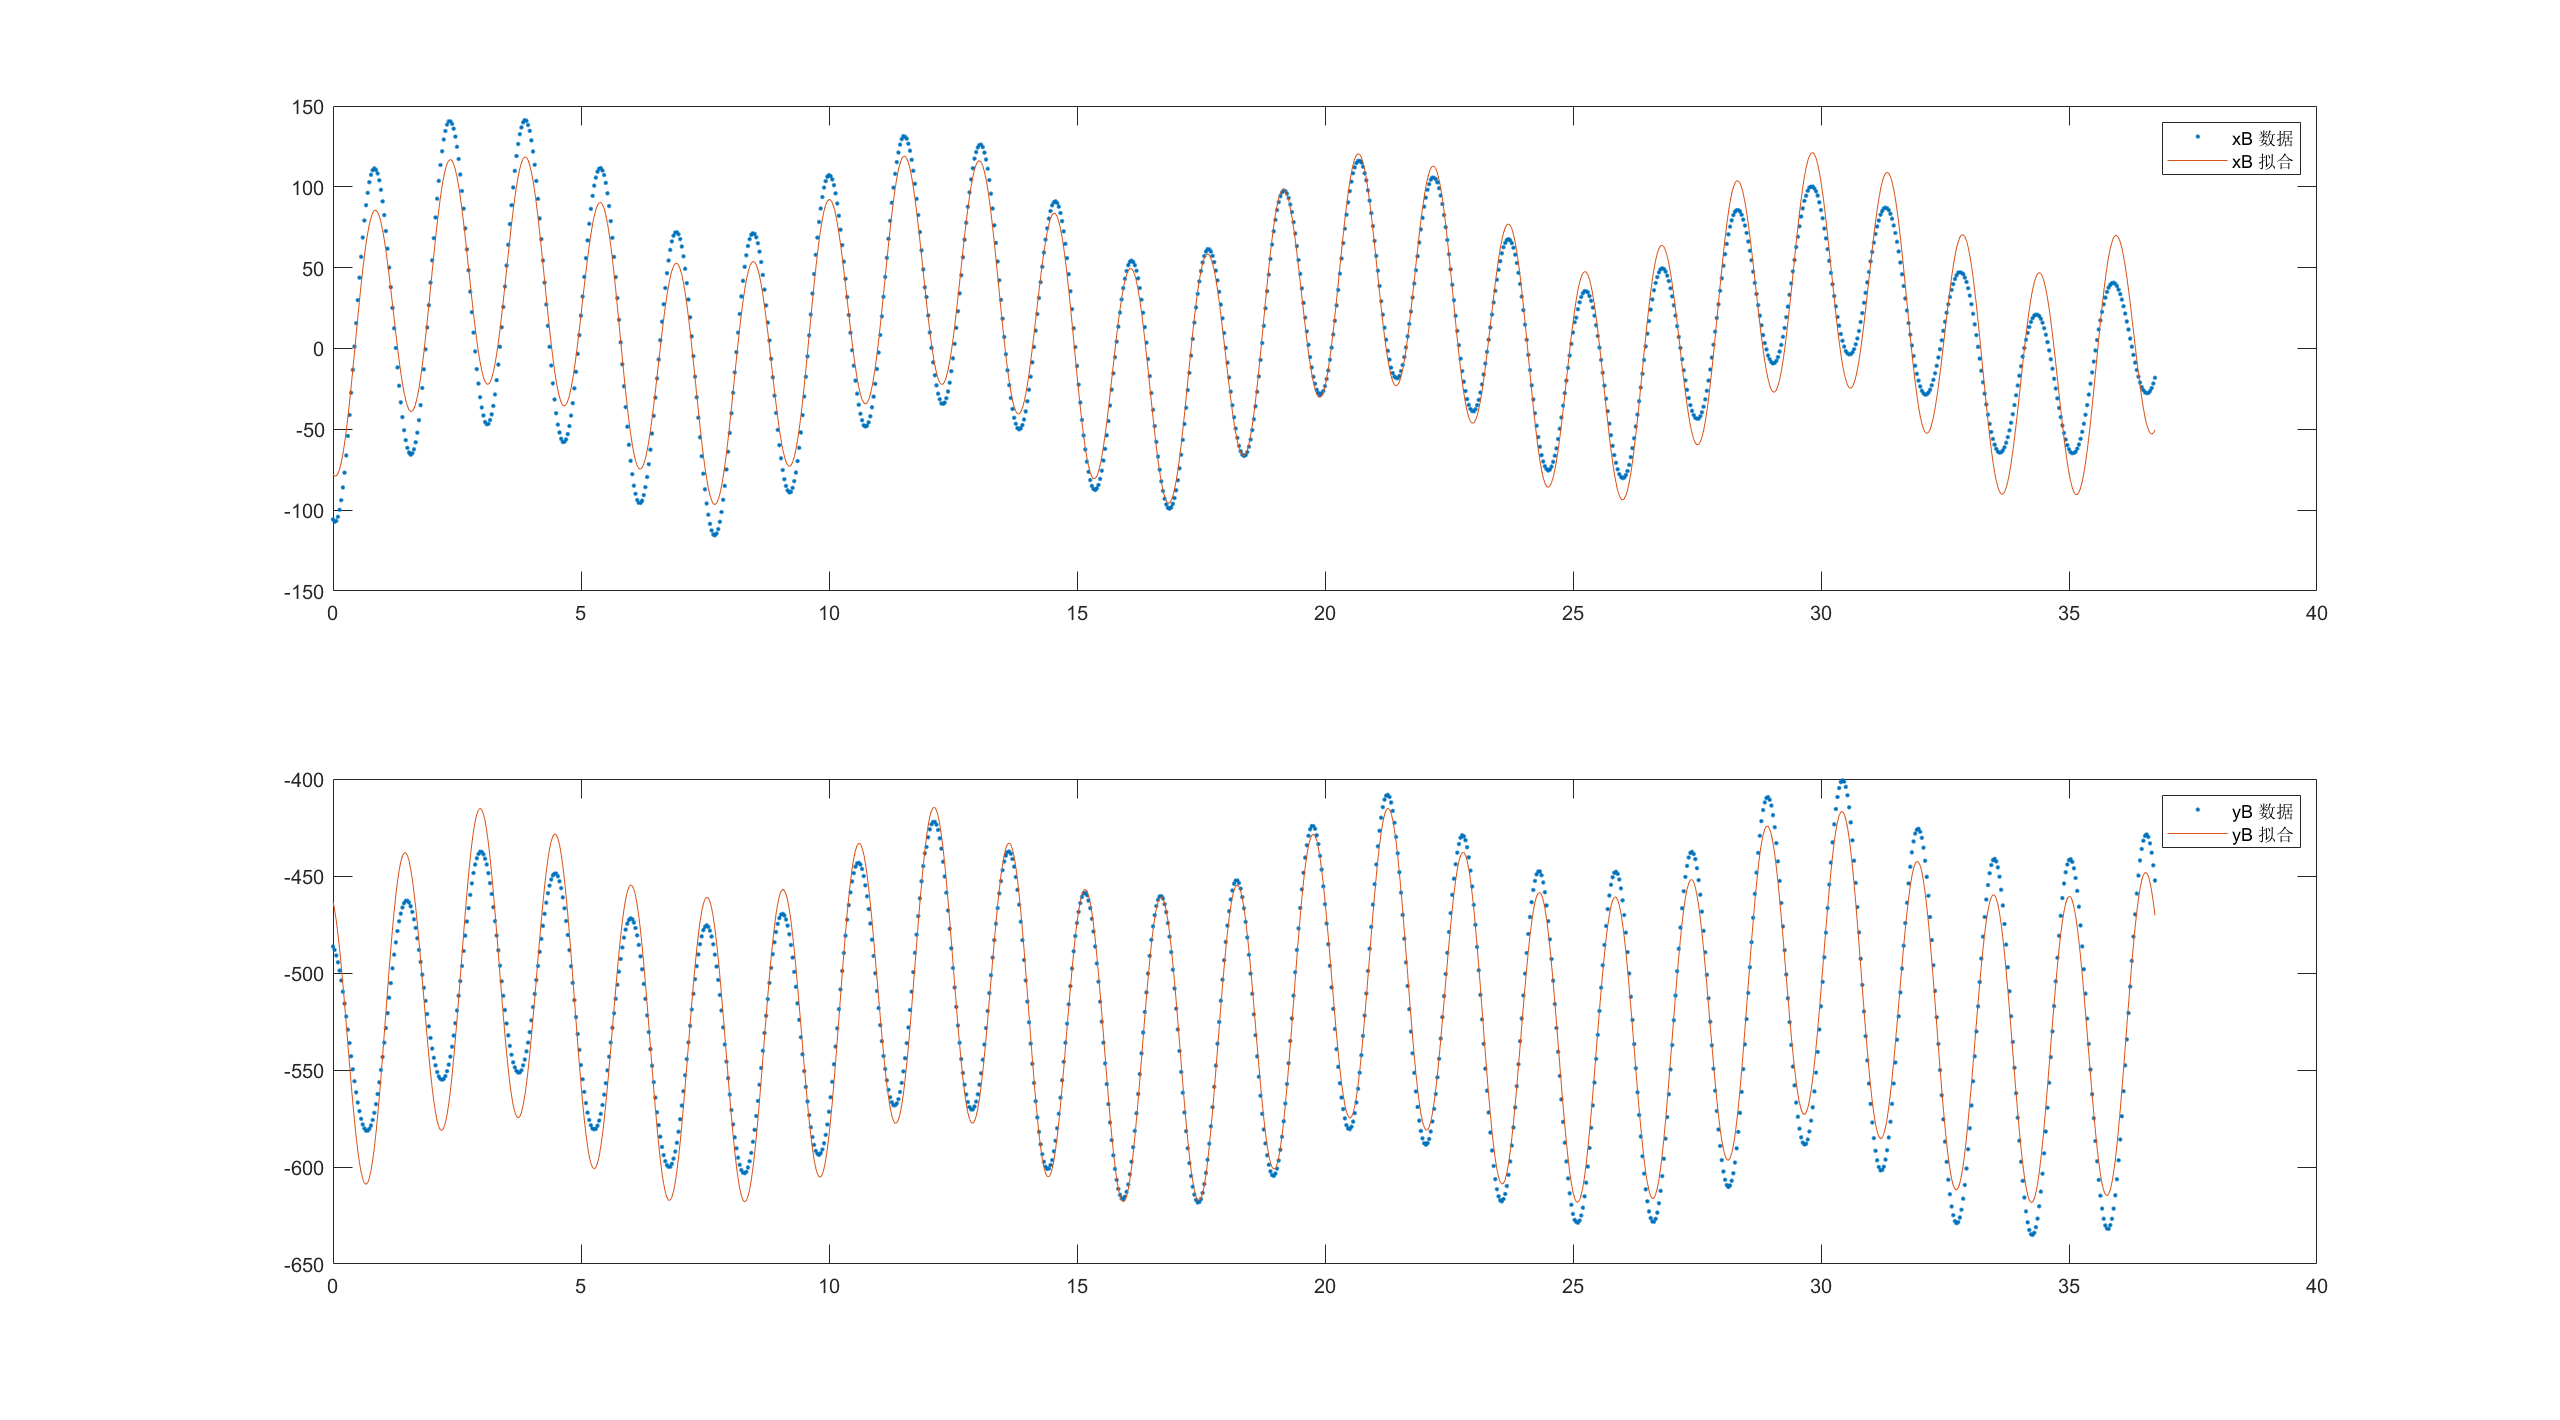
\includegraphics[width=0.9\textwidth]{Figs/Ex2.B.png}
            \vspace{-0.1cm}
            \caption{$B$点横纵坐标-时间拟合图}
        \end{figure}
        \item $A,B$两点反推得到的两组$(x_c(t),y_c(t))$的坐标轨迹图:
        \begin{figure}[H]
            \centering
            \begin{minipage}[t]{0.48\textwidth}
                \centering
                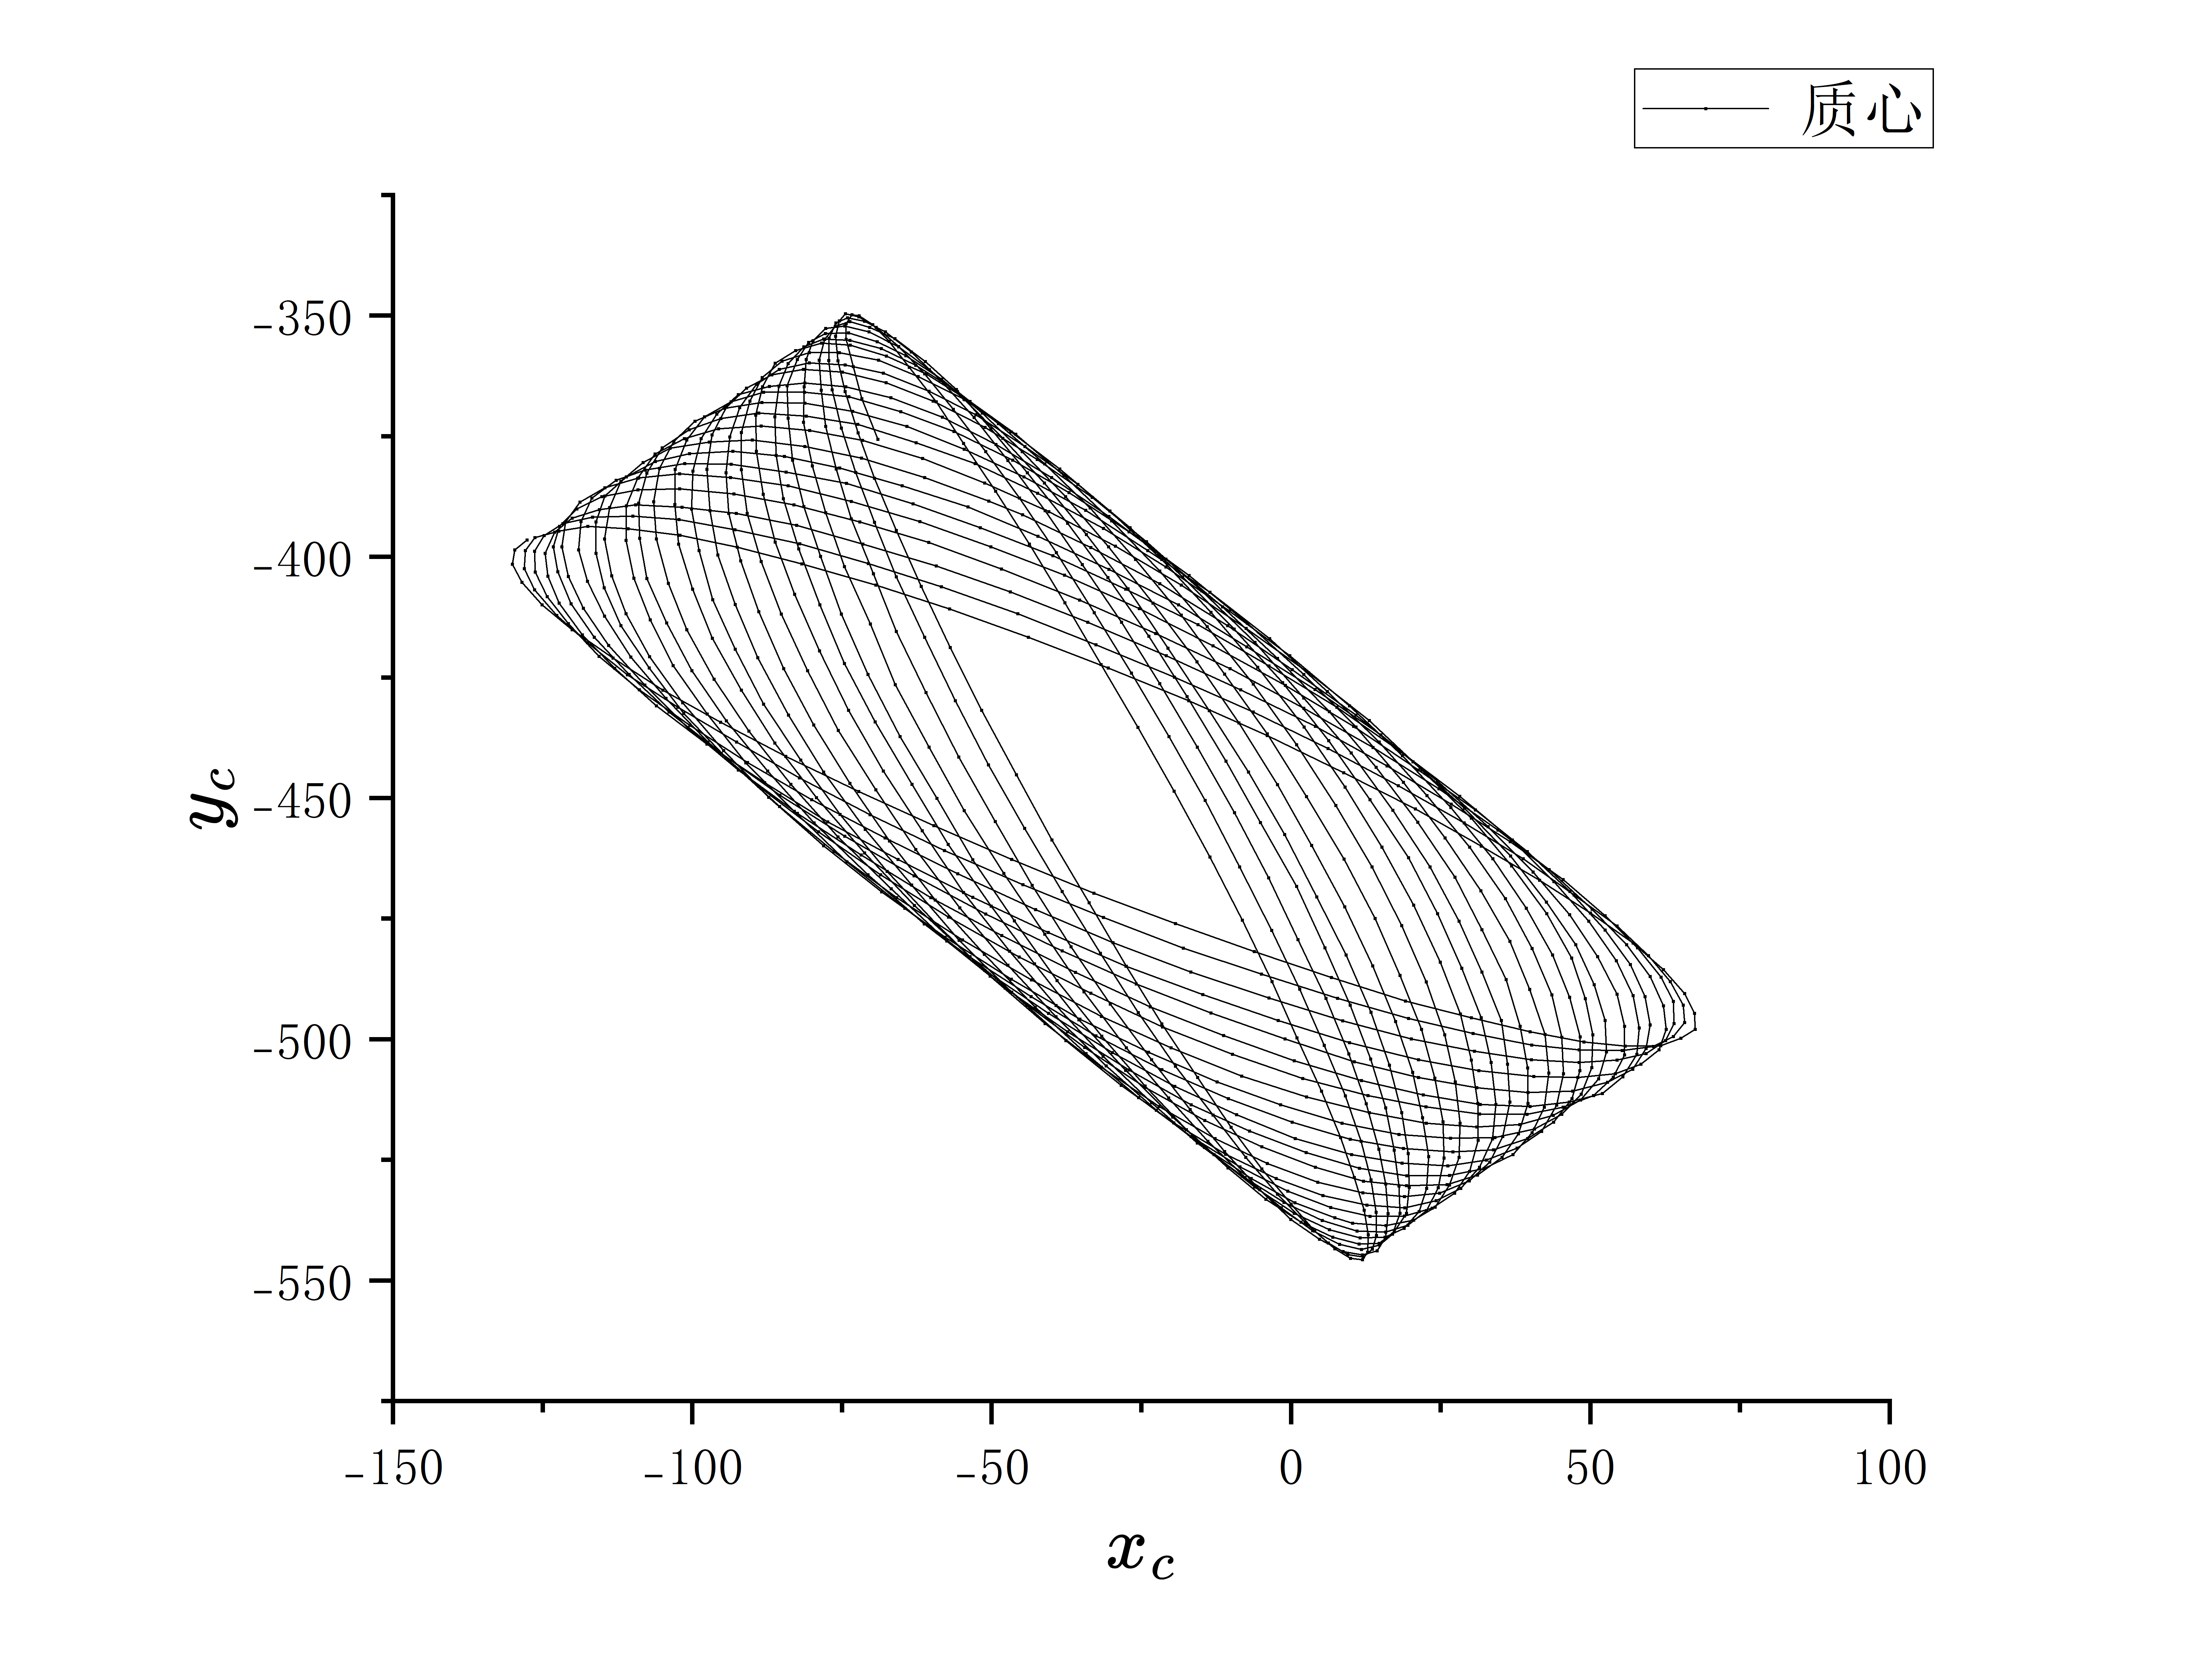
\includegraphics[width=\linewidth]{Figs/Ex2.A.c.png}
                \caption{$A$点反推的质心坐标轨迹图}
            \end{minipage}
            \hfill
            \begin{minipage}[t]{0.48\textwidth}
                \centering
                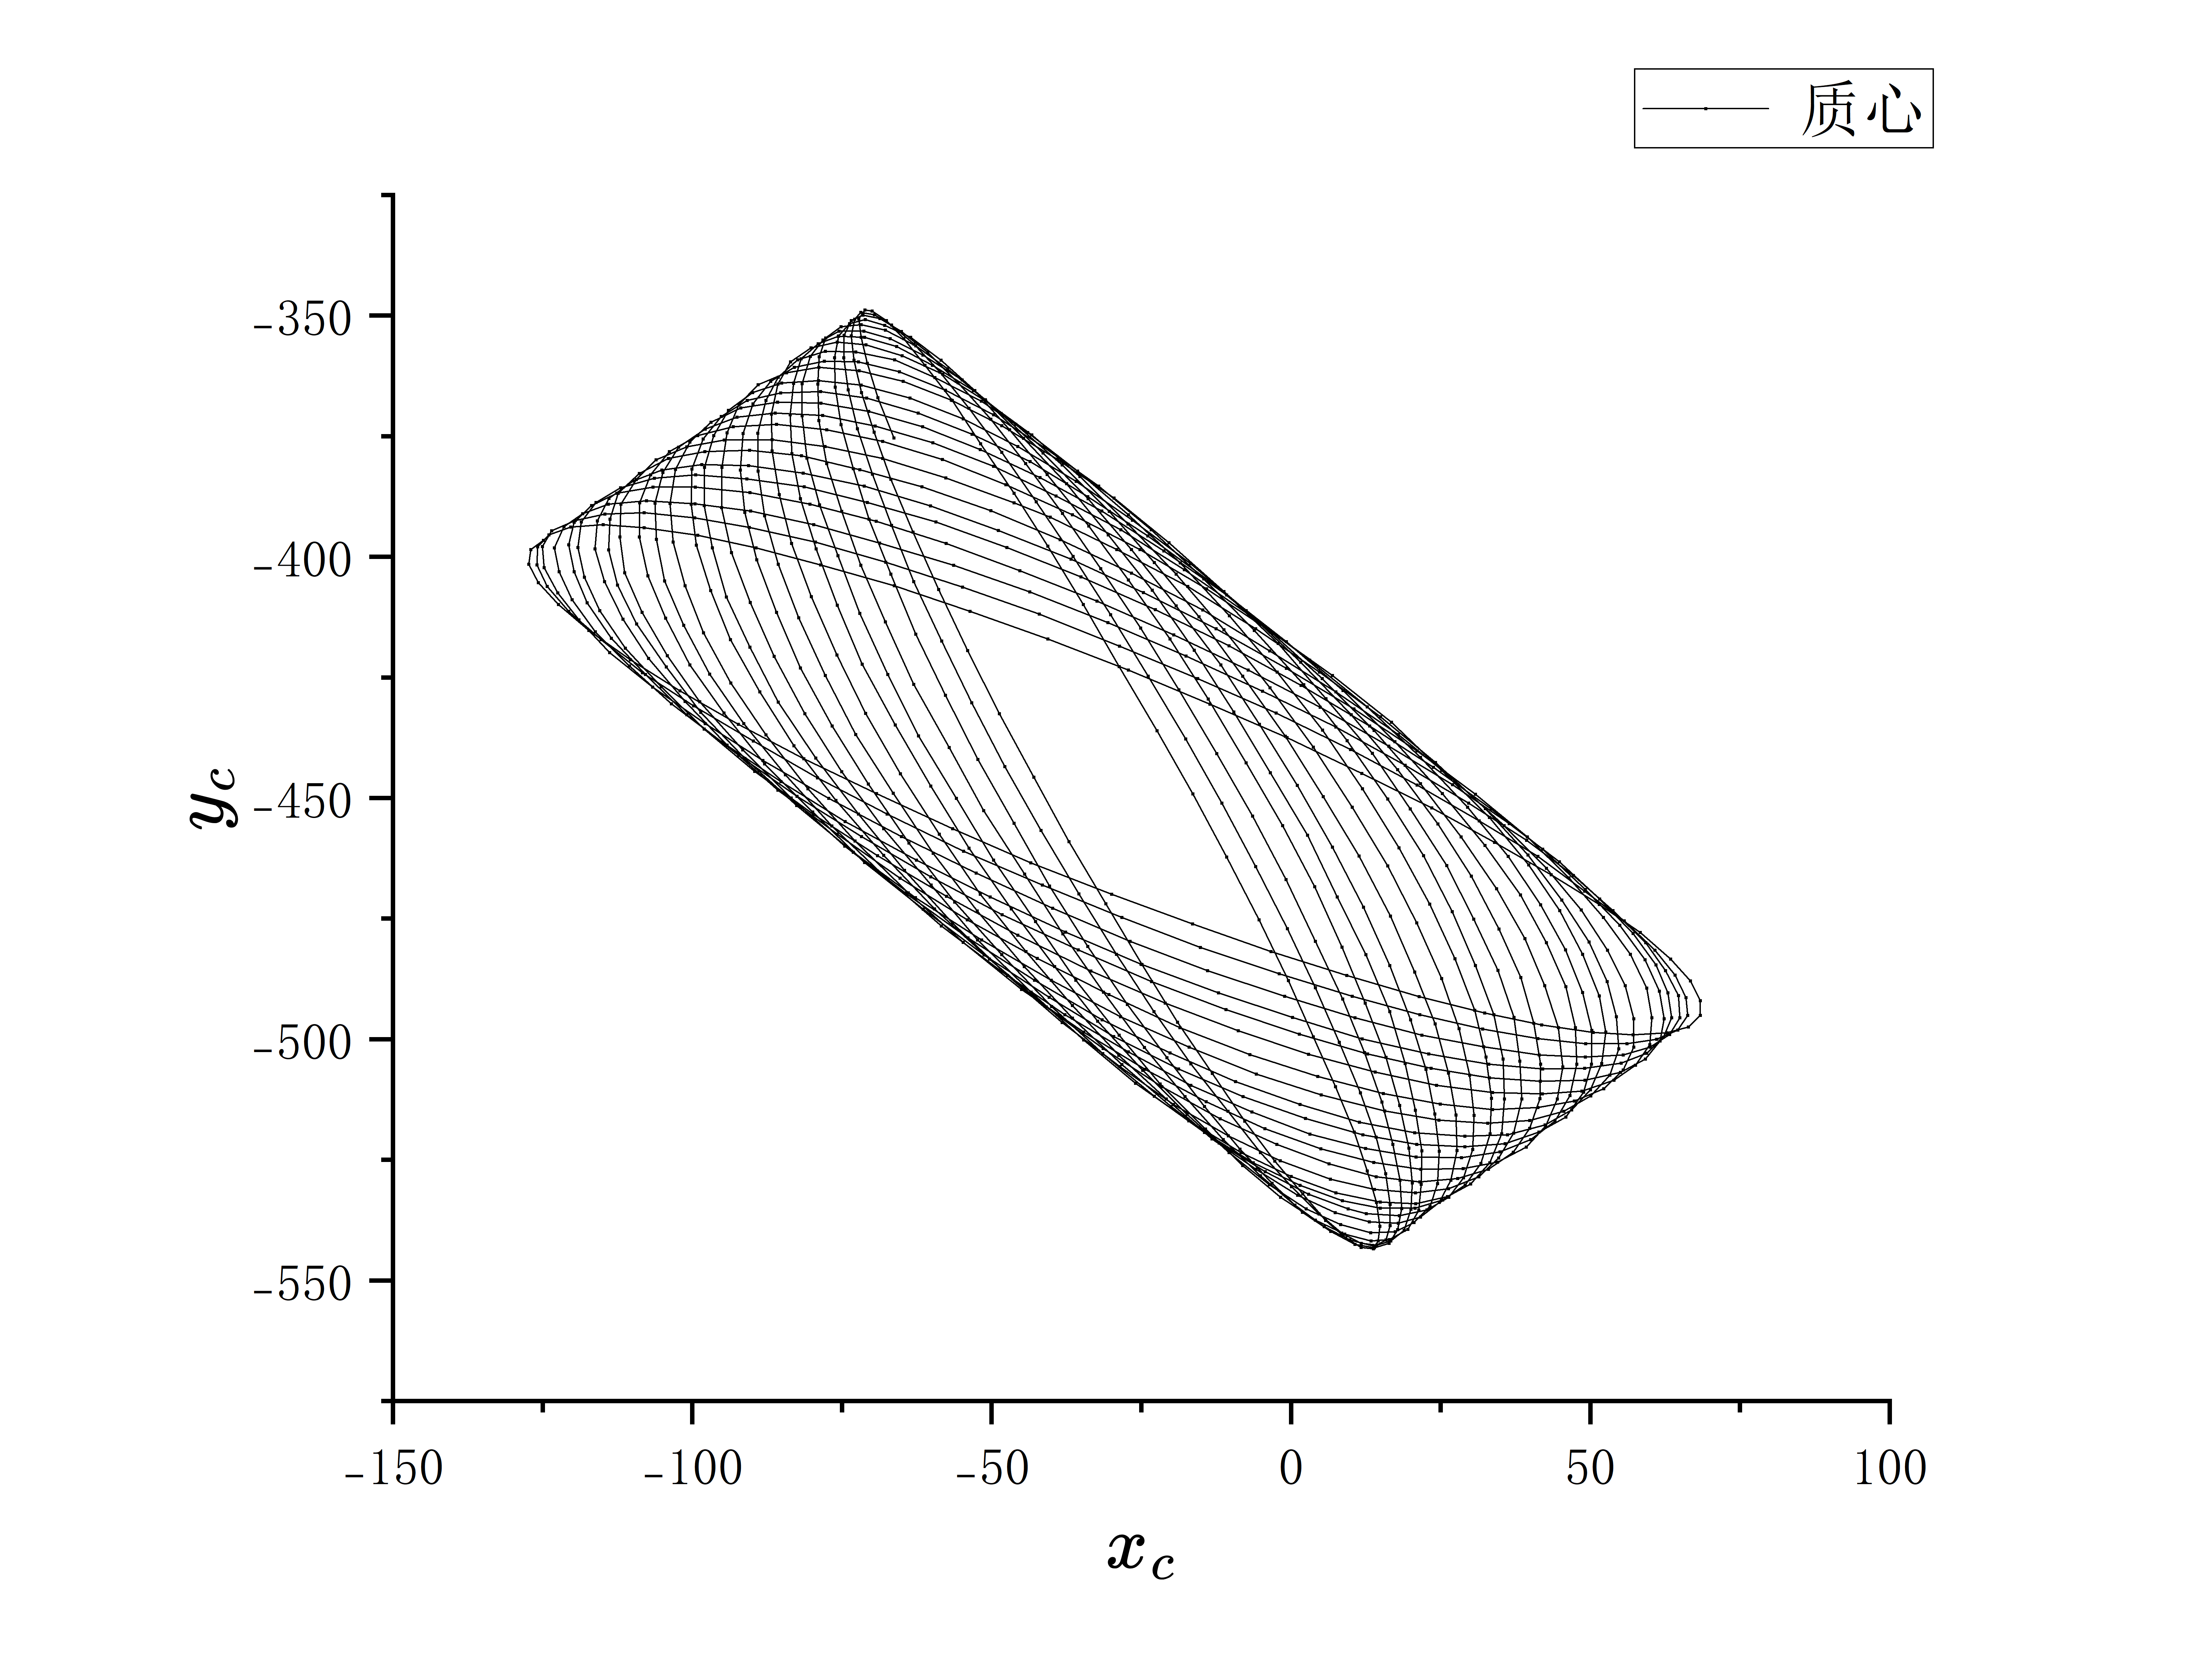
\includegraphics[width=\linewidth]{Figs/Ex2.B.c.png}
                \caption{$B$点反推的质心坐标轨迹图}
            \end{minipage}
        \end{figure}
    \end{enumerate}
    \item 对比分析:

    实验一中,测量出扭摆圆频率$\omega = 1.1947\,rad/s$,球面摆圆频率$\omega_g = 4.1060\,rad/s$,
    
    实验二中,测量出扭摆圆频率$\omega = 0.7048\,rad/s$,球面摆圆频率$\omega_g = 4.1177\,rad/s$,
    
    $\overline{\omega_g}=\dfrac{4.1060+4.1061+4.1177+4.1178}{4}=4.1119\,rad/s$
    
    根据绳长以及深圳的重力加速度$g=9.7887\,m/s^2$计算得到$\omega_{g_{ref}}=\sqrt{\dfrac{9.7887\,m/s^2}{0.5783\,m}}=4.1142\,rad/s$。
    
    经过对比,$\frac{|4.1177-4.1142|}{4.1142}\times100\%=0.085\%$,$\frac{|4.1060-4.1142|}{4.1142}\times100\%=0.199\%$,$\frac{|4.1119-4.1142|}{4.1142}\times100\%=0.056\%$,差距很小,可以认为球面摆的圆频率测量结果合理且添加圆盘后未影响球面摆的圆频率。比较两者扭摆部分的圆频率可以发现,添加圆盘后会使得扭摆的圆频率变小,与理论一致。
\end{enumerate}

\section*{七、误差分析}

\begin{enumerate}
    \item 使用tracker软件的自动追踪功能时,由于标识点并没有足够小,导致软件每次定位的位置有偏差,从而导致数据结果存在一定程度的误差;
    \item 球面摆存在进动,在拟合两点运动时忽略的其影响,对结果造成影响;
    \item 测量绳长时仪器带来误差;
    \item 扭摆与球面摆之间存在相互影响;
    \item 扭摆的转动中心并未与质心完美重合;
    \item 钢丝有弹性,摆动过程中会有微小的伸缩;
    \item 摆动过程中刚体在竖直方向有微小抖动;
    \item 拟合会导致数据不准确。
\end{enumerate}

\section*{八、实验结论}
\begin{enumerate}
    \item 验证了刚体的运动是球面摆运动和扭摆运动的复合,其拟合方程为;
        $$\left\{
        \begin{aligned}
            x(t)&=x_{c_0}+a\cos(\omega_{g}t+\varphi_x)+R\cos(\theta(t)+\theta_x) \\
            y(t)&=y_{c_0}+b\sin(\omega_{g}t+\varphi_y)+R\sin(\theta(t)+\theta_y)
        \end{aligned}
        \right.$$
        $$
        \text{其中:}\theta(t)=\theta_0+Asin(\omega t+\varphi)
        $$
    \item 改变刚体的质量只影响刚体扭摆的圆频率,两者呈负相关,不影响球面摆的圆频率。
    \item 测量得到此系统中刚体作扭摆运动的圆频率为$\omega=1.1947\,rad/s$,刚体作球面摆运动的圆频率为$\omega_g=4.1119\,rad/s$,其相对误差为$0.056\%$。
\end{enumerate}

\section*{九、参考文献}

\begingroup  % 去掉thebibliography环境自带的“参考文献”标题
\renewcommand{\section}[2]{} 
\begin{thebibliography}{99}
    \bibitem{ref1} 实验讲义,18.切变模量的测量-2025
    \bibitem{ref2} 杨仲准. 台湾中原大学 Tracker 软件安装与使用教学 [EB/OL]. 中原大学物理实验室, \\ http://www.phys.nthu.edu.tw/~gplab/file/resources/\\How\%20to\%20use\%20Tracker-CYCU\_CCYang.pdf
    \bibitem{ref3} 周子栋,邵明珍,王才林,曾孝奇,张欢,利用扭摆实验探究简谐运动规律,物理实验,2022,42(2):53-57.
\end{thebibliography}
\endgroup

\section*{十、小组分工}

\begin{enumerate}
    \item 王悦安:组长、理论推导、实验操作、数据记录;
    \item 钱家祺:汇报展示、报告撰写、理论推导;
    \item 杨越文:实验操作、数据记录、数据处理、报告撰写;
    \item 秦炜卓:幻灯片制作、实验操作、数据记录。
\end{enumerate}

\end{document}